\documentclass{article}
\usepackage{amsmath}
\usepackage{geometry}
%\usepackage[]{mcode}
\usepackage{graphicx}
\usepackage{float}
\usepackage{placeins}
\usepackage{gensymb}
\usepackage{subfig}
\usepackage[space]{grffile}
% Allow \href{http://url}{name}
\usepackage{hyperref}
\usepackage{xcolor}
\usepackage{float}

\hypersetup{
    colorlinks=true,
    linkcolor={red!50!black},
    citecolor={blue!50!black},
    urlcolor={blue!80!black}
}

\geometry{
left = 1.25in,
lmargin = 1.25in,
inner = 1.25in,
right = 1.25in,
rmargin = 1.25in,
outer = 1.25in,
top = 1in,
tmargin = 1in,
bottom = 1in,
bmargin = 1in,
}

\begin{document}

\title{Inverted Pendulum Controllers}
\author{Garrett Wilson and Nathan Zimmerly \\ \\
ENGR 352}
\maketitle

\clearpage
\tableofcontents
\pagebreak

\section{PID Controller}
The derivations below are based on the following diagrams

\begin{figure}[H]
\centering
\subfloat[Pendulum System]{{
	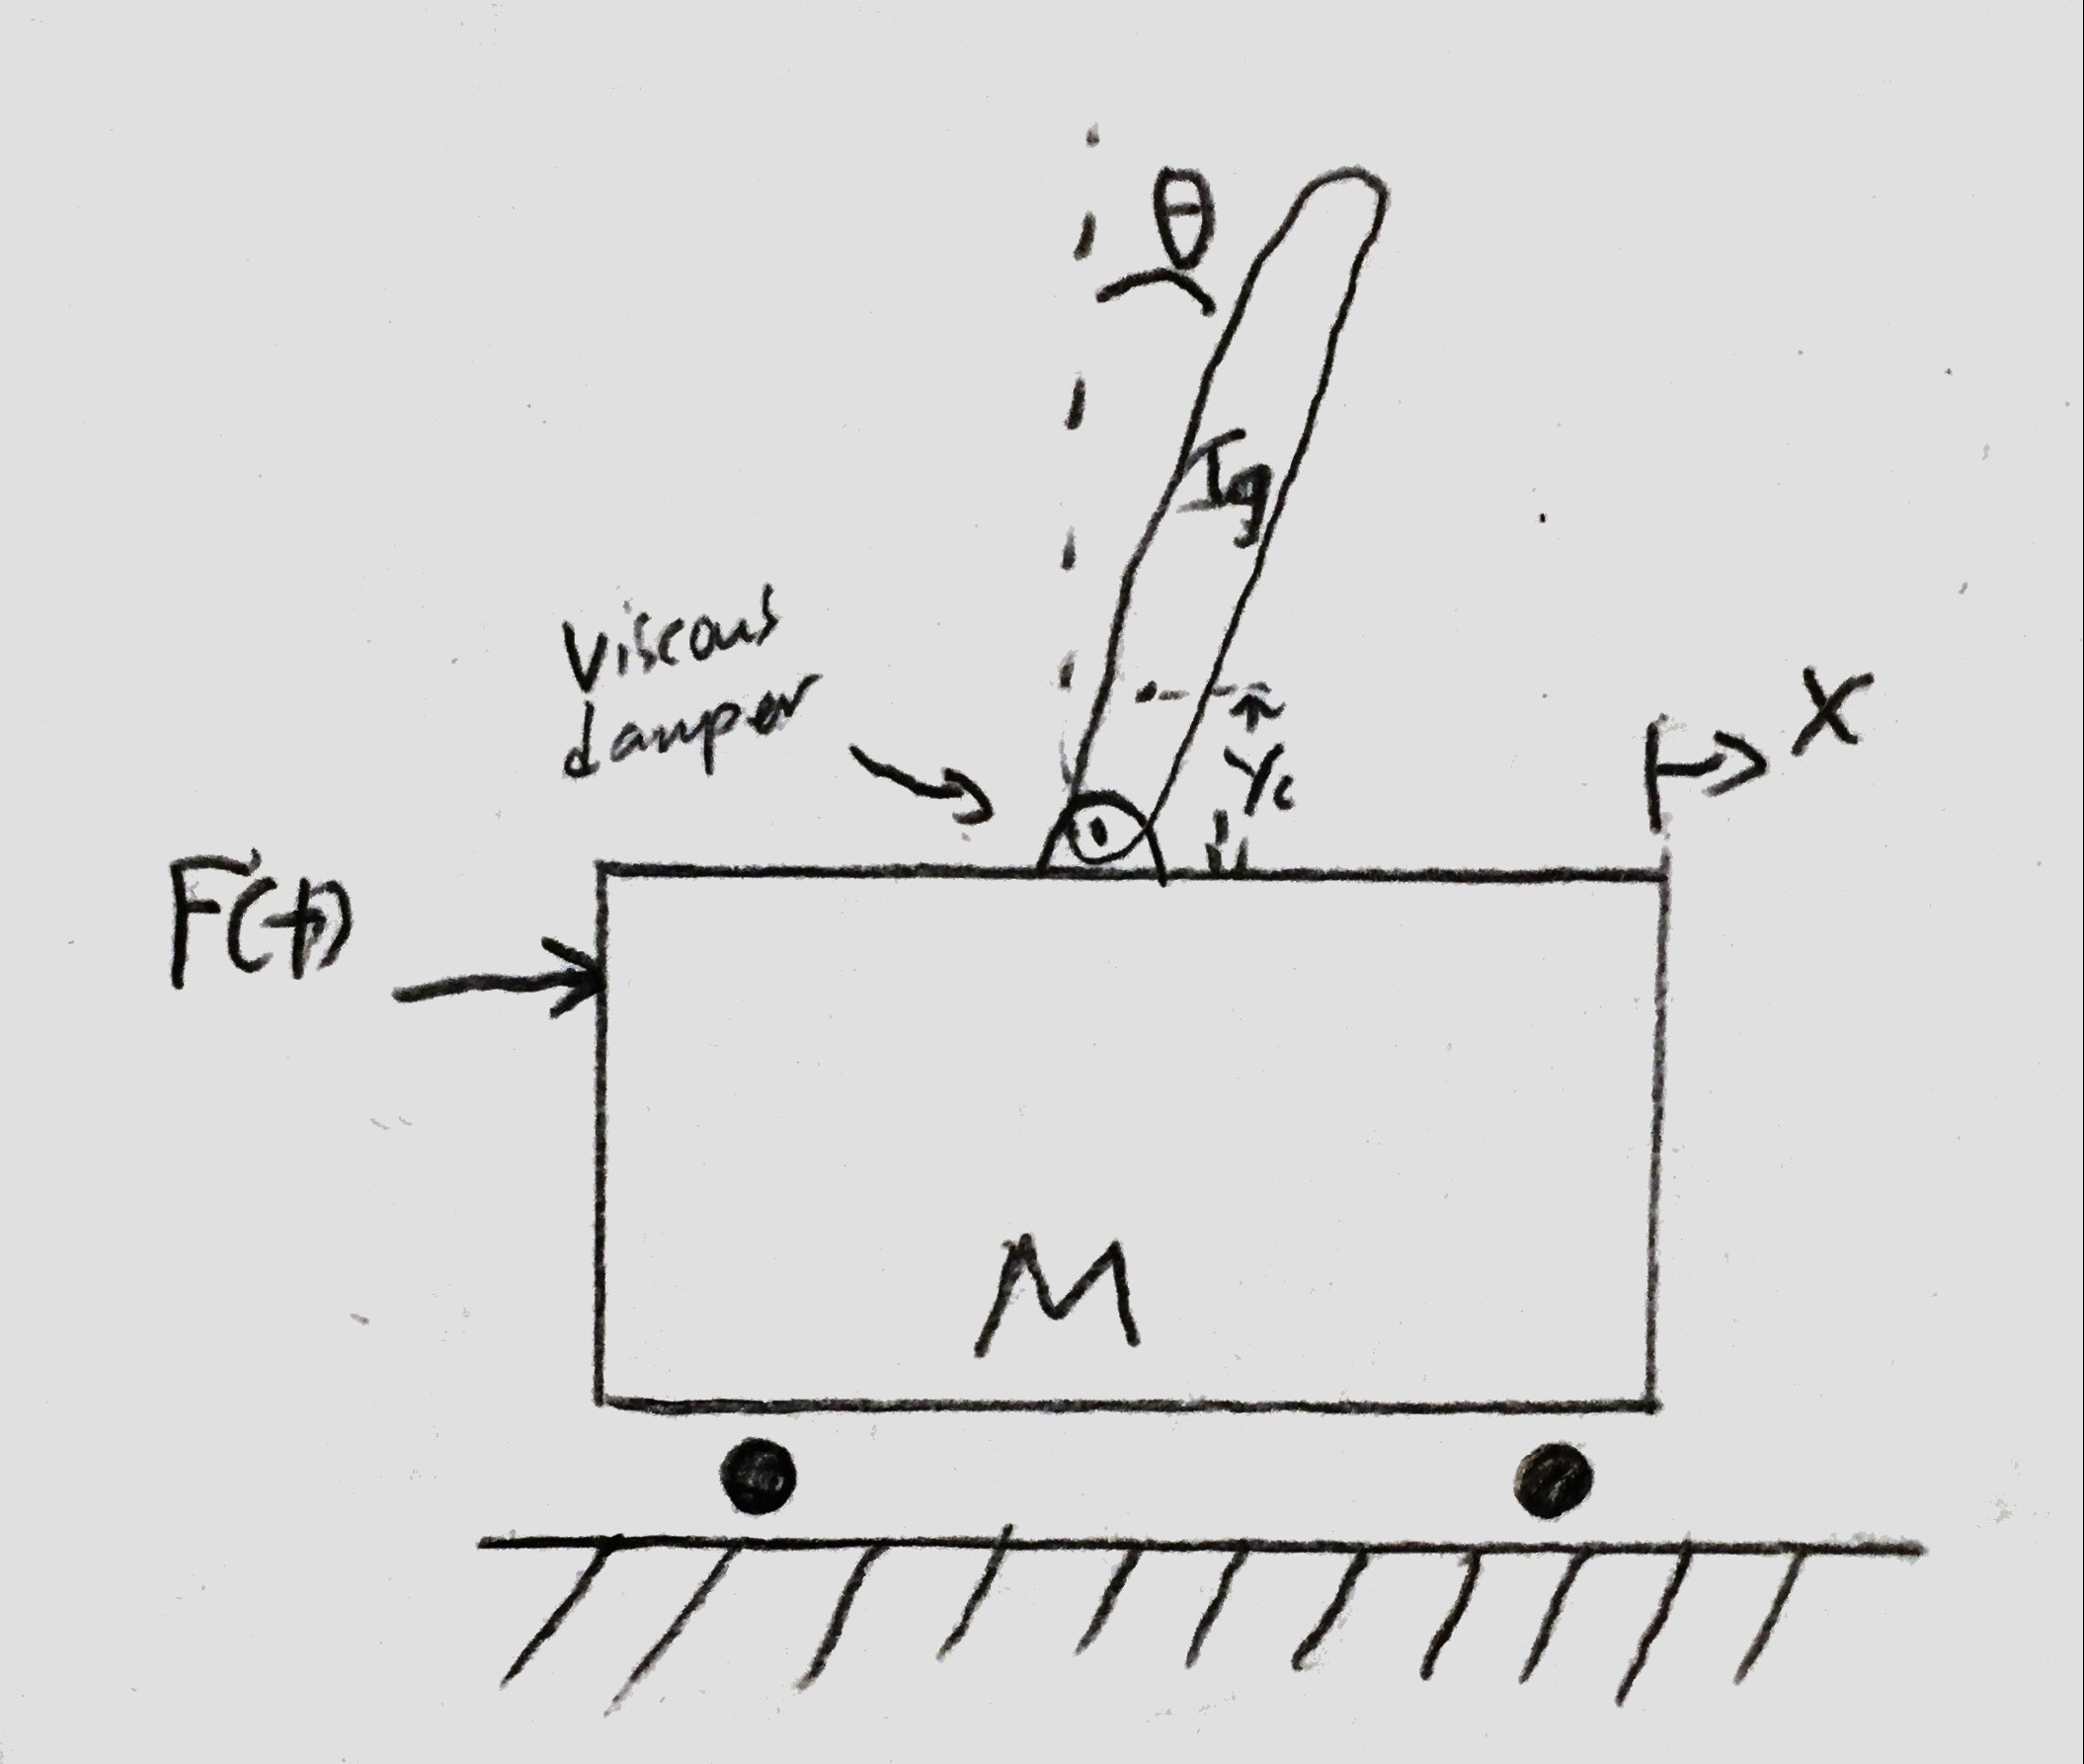
\includegraphics[width=0.5\linewidth]{Inverted Pendulum Diagram}
	\label{fig:ipd}
}}
	\subfloat[Pendulum KD]{{
	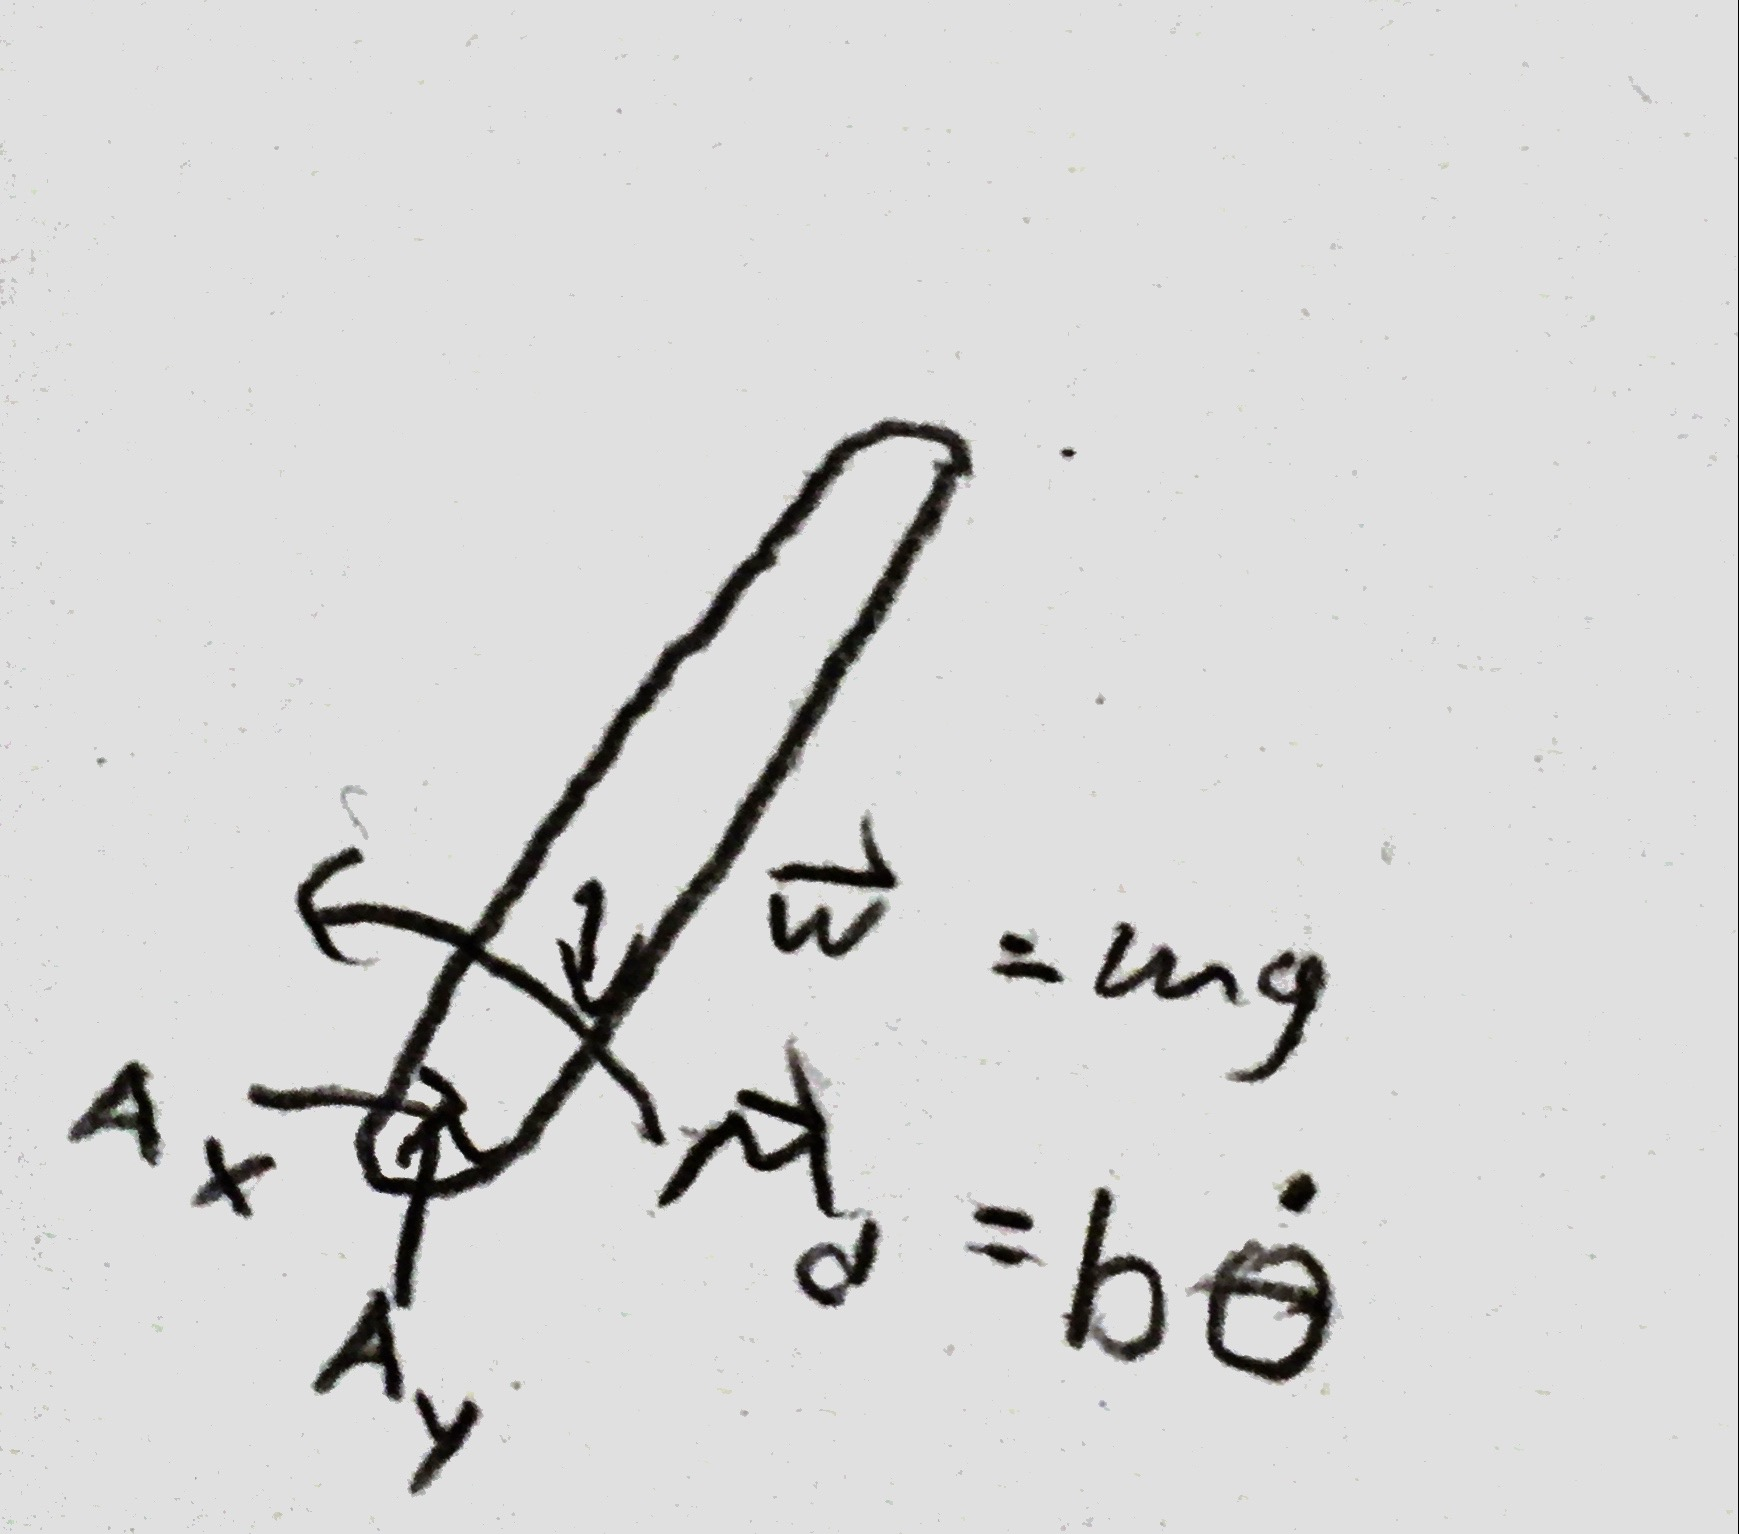
\includegraphics[width=0.5\linewidth]{Pendulum KD}
	\label{fig:pkd}
}}
\caption{Pendulum Diagrams}
\end{figure}

\begin{figure}[H]
\centering
\subfloat[Cart FBD]{{
	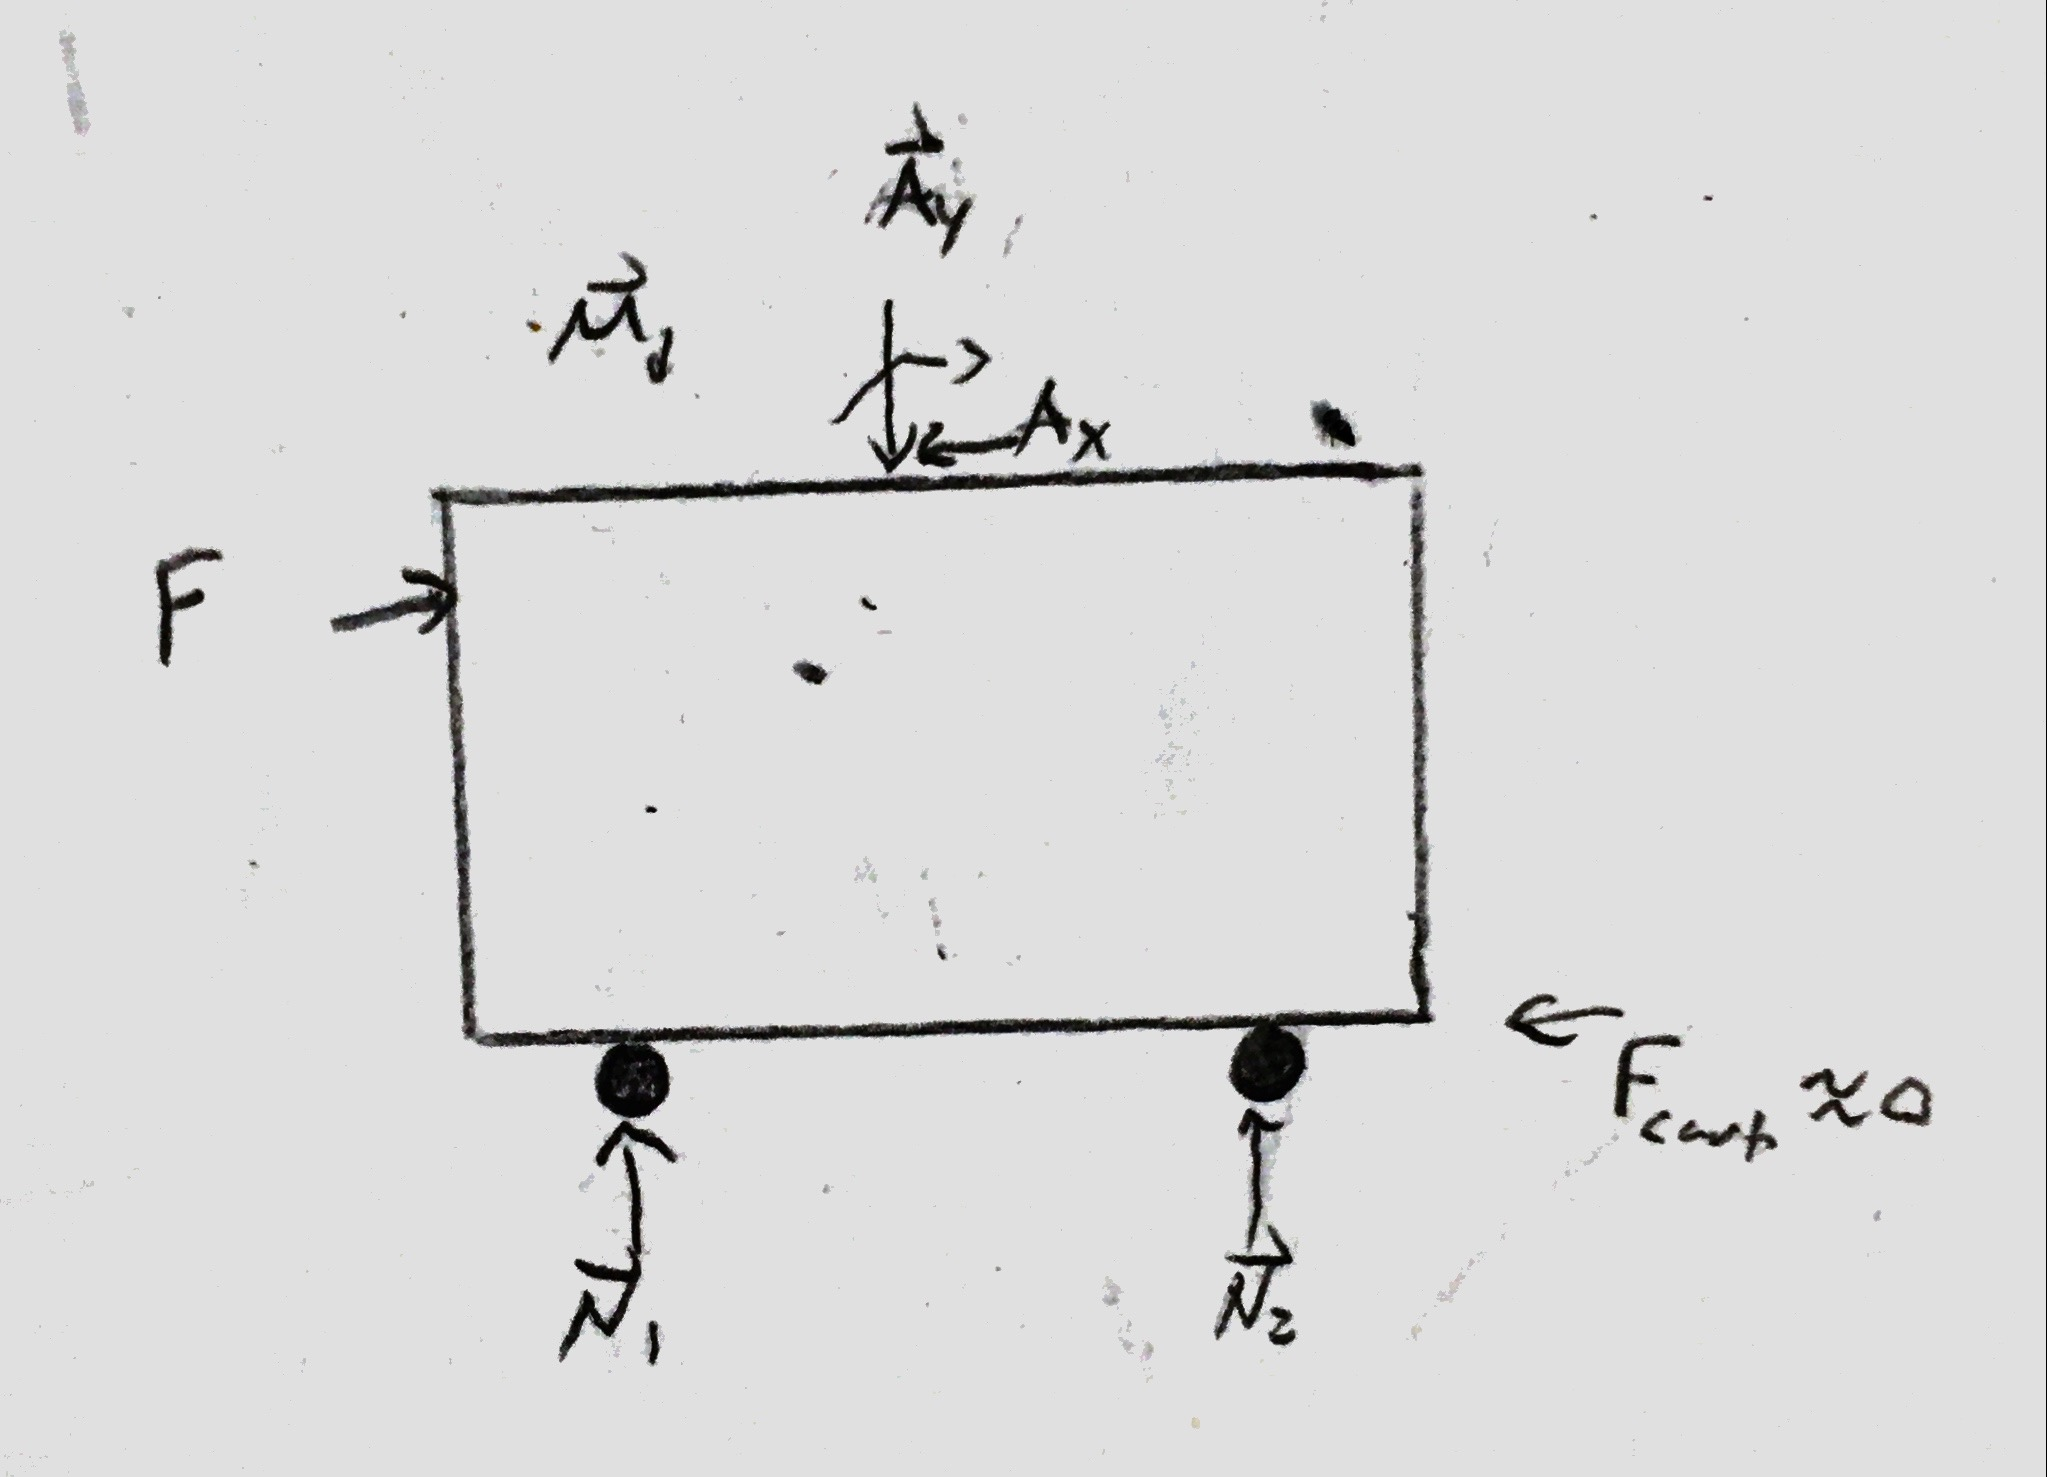
\includegraphics[width=0.5\linewidth]{Cart FBD}
	\label{fig:cfbd}
}}
	\subfloat[Pendulum FBD]{{
	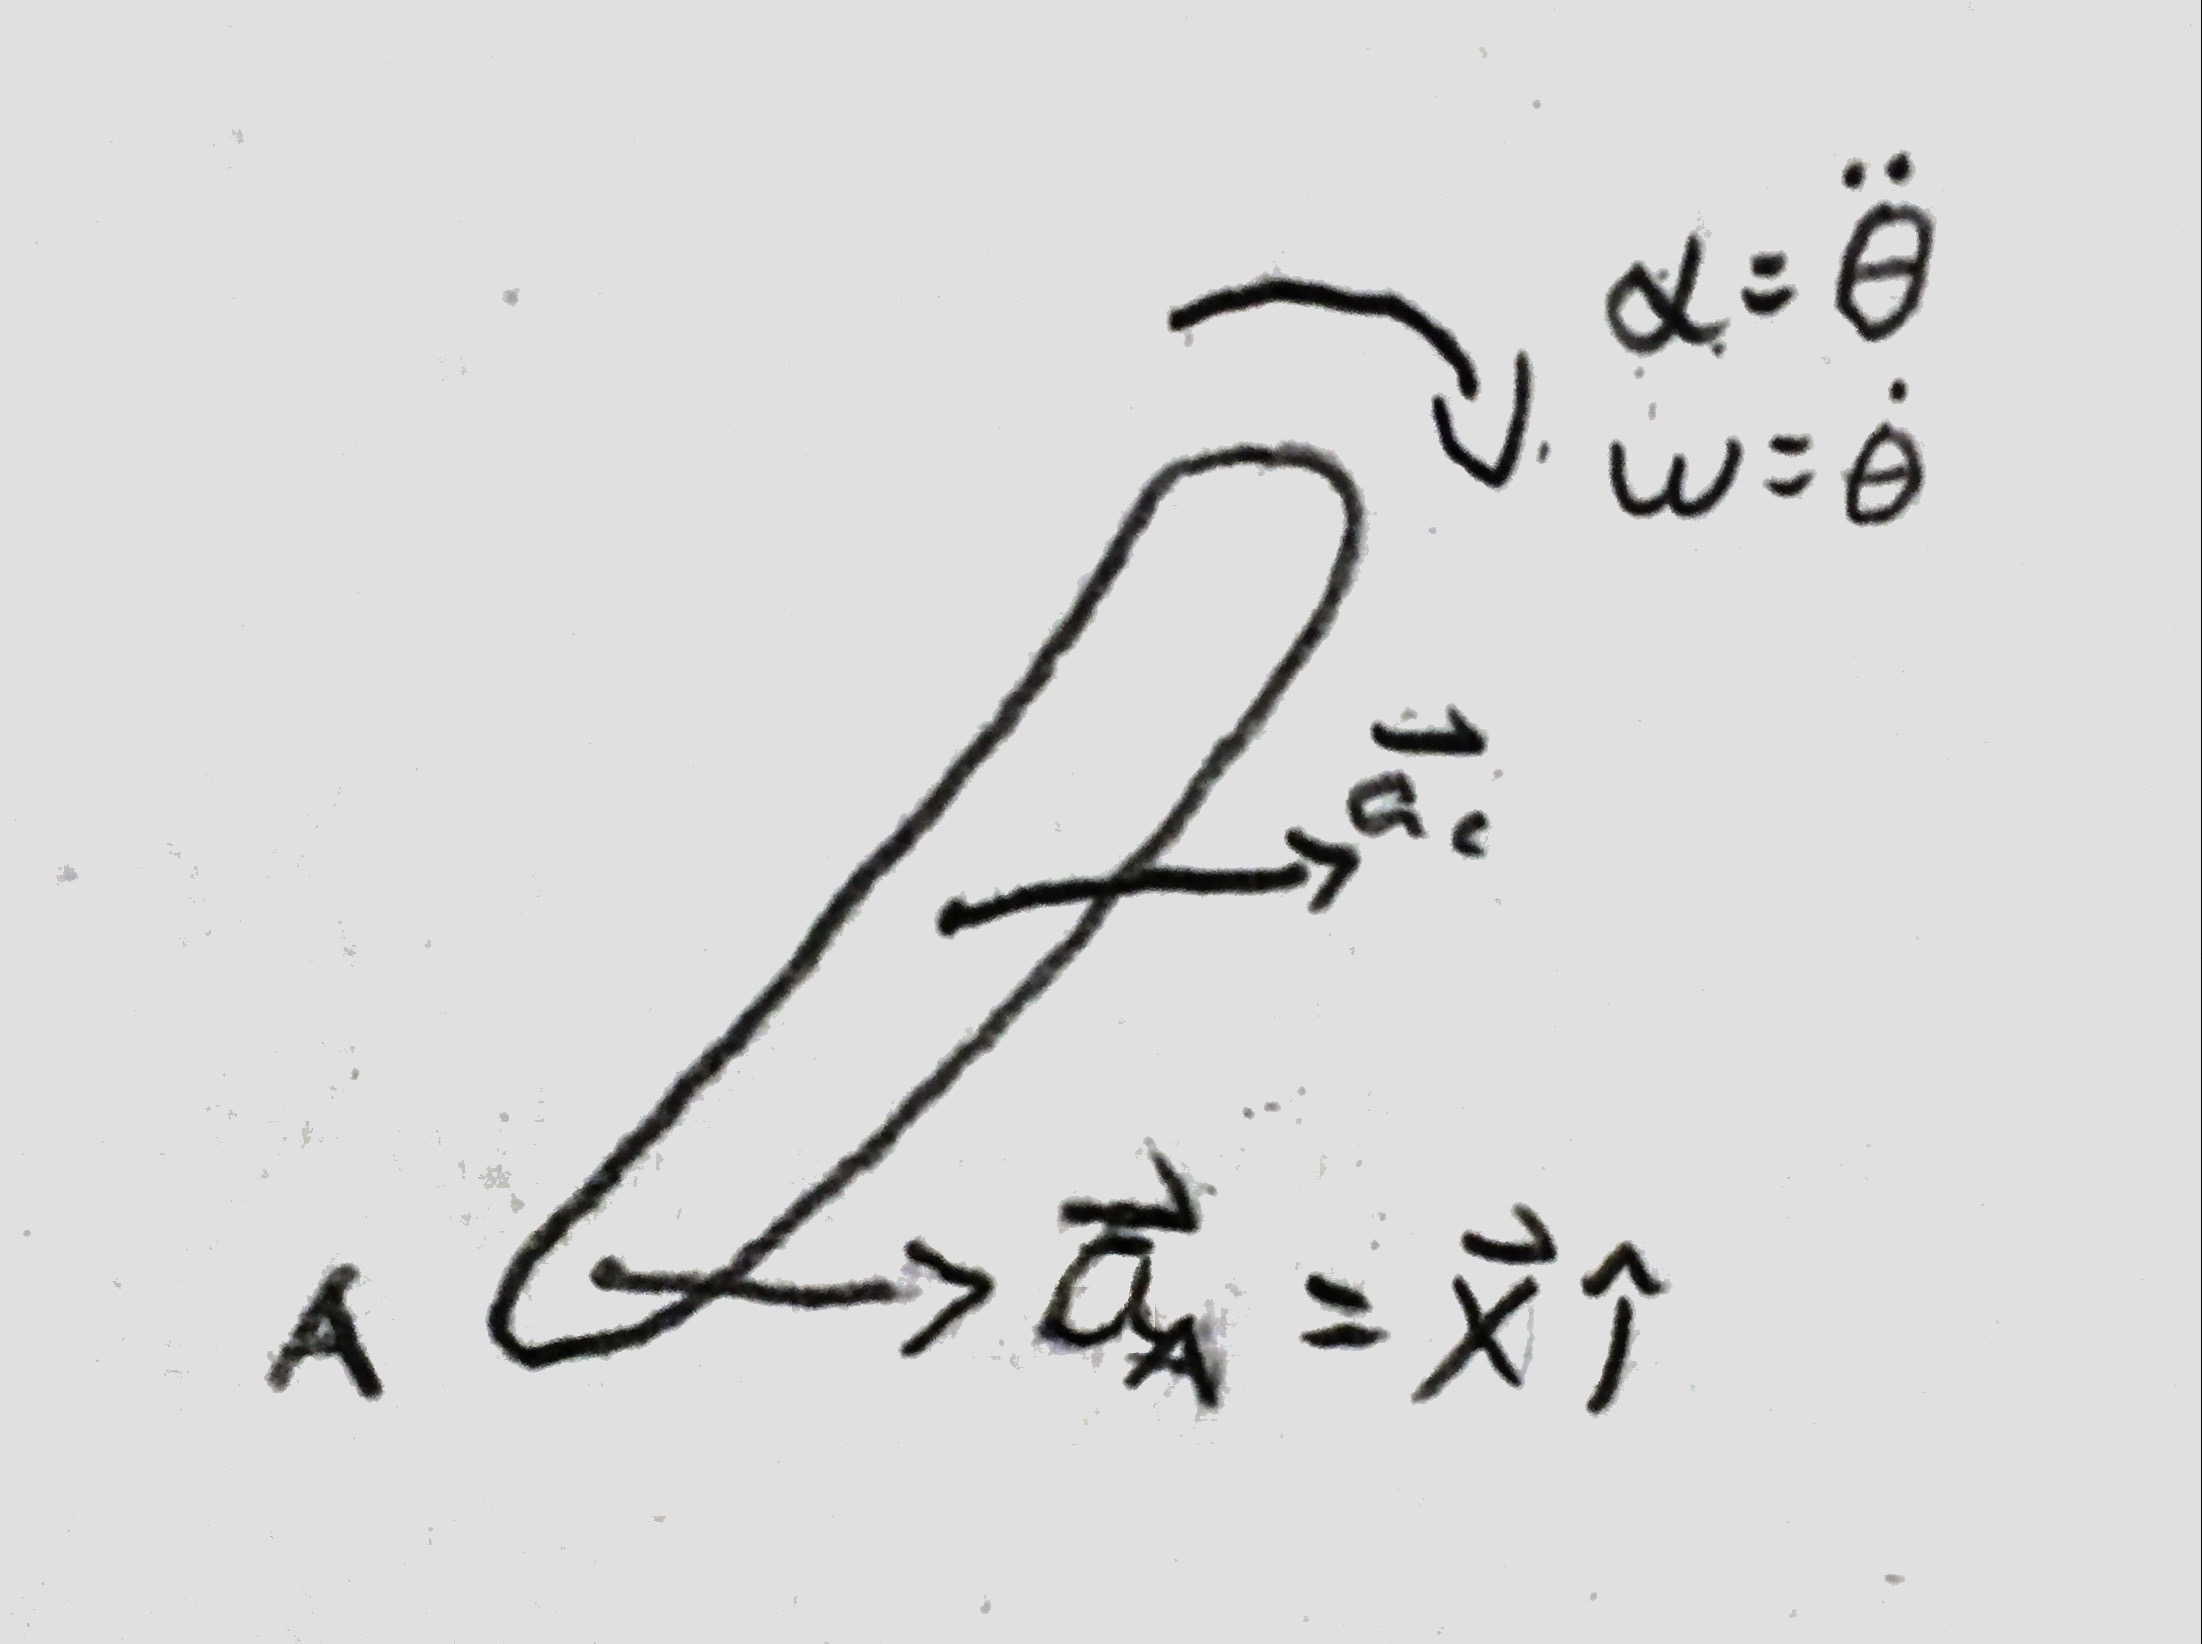
\includegraphics[width=0.5\linewidth]{Pendulum FBD}
	\label{fig:pfbd}
}}
\caption{Free Body Diagrams}
\end{figure}

\subsection{Transfer Function of $\theta$ / F Without Friction Derivation}
Below is the derivation of the transfer function with an input of F and an output of $\theta$.


\begin{equation} 
\label{eqn1}
\ddot \theta (I+m y_c^2)+\ddot x (m y_c)+b \dot \theta - m g y_c \theta = 0 
\end{equation}


\begin{equation} 
\label{eqn2}
\ddot \theta(m y_c) + \ddot x(M+m) = F
\end{equation}

%\\
Laplace transforms of equations \ref{eqn1} and \ref{eqn2} gives

\begin{equation} 
\label{eqn1l}
\theta (I+m y_c^2) s^2+ X (m y_c) s^2+b \theta s - m g y_c \theta = 0 
\end{equation}


\begin{equation}  
\label{eqn2l}
\theta (m y_c) s^2+ X (M+m) s^2= F
\end{equation}

%\\
Next, solving \ref{eqn2l} for x and substituting it into \ref{eqn1l}

\begin{equation}  
\label{eqn2lb}
X = \frac{F - \theta (m y_c) s^2}{(M+m) s^2}
\end{equation}

\begin{equation} 
\label{eqn3}
\theta (I+m y_c^2) s^2+ \frac{(F - \theta (m y_c) s^2)(m y_c) s^2}{(M+m) s^2} + b \theta s - m g y_c \theta = 0 
\end{equation}

Simplifying \ref{eqn3} leads to


\begin{equation} 
\label{eqn3}
\theta (I+m y_c^2) s^2+ \frac{F m y_c}{(M+m)} -\frac{\theta (m y_c)^2 s^2}{(M+m)} + b \theta s - m g y_c \theta = 0 
\end{equation}

\begin{equation} 
\label{eqn3b}
\theta [(I+m y_c^2) s^2 - \frac{(m y_c)^2 s^2}{(M+m)} + b s - m g y_c] +\frac{F m y_c}{(M+m)}  = 0 
\end{equation}

\begin{equation} 
\label{eqn3c}
\theta [(I+m y_c^2) s^2 - \frac{(m y_c)^2 s^2}{(M+m)} + b s - m g y_c] = -\frac{F m y_c}{(M+m)} 
\end{equation}

\begin{equation} 
\label{eqn3d}
\theta [(I+m y_c^2)(M+m) s^2 - (m y_c)^2 s^2 + b s (M+m) - m g y_c (M+m) ] = -F m y_c
\end{equation}

\begin{equation} 
\label{eqn3e}
\frac{\theta}{F} = \frac{-m y_c}{(I+m y_c^2)(M+m) s^2 - (m y_c)^2 s^2 + b s (M+m) - m g y_c (M+m)}
\end{equation}

\begin{equation} 
\label{eqntf1}
\frac{\theta}{F} = \frac{-m y_c}{[(I+m y_c^2)(M+m) - (m y_c)^2]s^2 + b (M+m) s - m g y_c (M+m)}
\end{equation}

Equation \ref{eqntf1} is the transfer function of $\theta$ / F without friction.

\subsection{Transfer Function X / $\theta$ Derivation}
We are deriving this transfer function so that we can plot the position of the cart as the system respondsto the input impulse properly.
\\
\\
Using \ref{eqn1l}

\begin{equation} 
\label{eqn4}
X (m y_c) s^2 = -\theta [(I+m y_c^2) s^2+b s - m g y_c] = 0 
\end{equation}

\begin{equation} 
\label{eqntf2}
\frac{X}{\theta} = \frac{-[(I+m y_c^2) s^2+b s - m g y_c]}{(m y_c) s^2} 
\end{equation}

Equation \ref{eqntf2} is the transfer function of X / $\theta$.



\subsection{Transfer Function of $\theta$ / F with Friction Derivation}

Below is the derivation of the transfer function with an input of F and an output of $\theta$.

\begin{equation} 
\label{eqn5}
\ddot \theta (I+m y_c^2)+\ddot x (m y_c)+b \dot \theta - m g y_c \theta = 0 
\end{equation}

\begin{equation} 
\label{eqn6}
\ddot \theta(m y_c) + \ddot x(M+m) = F+ F_{fric}
\end{equation}

These equations are equivalent to \ref{eqn1} and \ref{eqn2} except \ref{eqn2} has $F_{fric}$ added.

\begin{equation}
\label{eqn7}
F_{fric} = - b_cart \dot x
\end{equation}

Substituting \ref{eqn7} into \ref{eqn6}

\begin{equation} 
\label{eqn8}
\ddot \theta(m y_c) + \ddot x(M+m) = F - b_{cart} \dot x
\end{equation}

Laplace Transforms of \ref{eqn5} and \ref{eqn8} give

\begin{equation} 
\label{eqn5l}
\theta (I+m y_c^2) s^2+ X (m y_c) s^2+b \theta s - m g y_c \theta = 0 
\end{equation}

\begin{equation} 
\label{eqn8l}
\theta (m y_c) s^2+ X (M+m) s^2= F - b_{cart} X s
\end{equation}

Solving \ref{eqn8l} for X and solving substituting the result into \ref{eqn5l} gives

\begin{equation} 
\label{eqn8lb}
X [(M+m) s^2 + b_{cart} s]= F - \theta(m y_c) s^2
\end{equation}

\begin{equation} 
\label{eqn8lc}
X = \frac{F - \theta(m y_c) s^2}{(M+m) s^2 + b_{cart} s}
\end{equation}

\begin{equation} 
\label{eqn9}
\theta (I+m y_c^2) s^2+  \frac{[F - \theta(m y_c) s^2] m y_c s^2}{(M+m) s^2 + b_{cart} s}+b \theta s - m g y_c \theta = 0 
\end{equation}

Solving \ref{eqn9} for the transfer function

\begin{multline} 
\label{eqn9b}
\theta (I+m y_c^2) s^2 [(M+m) s^2 + b_{cart} s]+ F m y_c s^2 - \theta(m y_c)^2 s^4 \\ 
+ b \theta s [(M+m) s^2 + b_{cart} s]- m g y_c \theta [(M+m) s^2 + b_{cart} s]= 0 
\end{multline}

\begin{multline} 
\label{eqn9c}
\theta [(I+m y_c^2) s^2 ((M+m) s^2 + b_{cart} s) - (m y_c)^2 s^4 + b s ((M+m) s^2 \\+ b_{cart} s)
- m g y_c ((M+m) s^2 + b_{cart} s)] = -F m y_c s^2
\end{multline}

\begin{multline} 
\label{eqn9d}
\frac{\theta}{F} = (-m y_c s^2)/((I+m y_c^2) s^2 ((M+m) s^2 + b_{cart} s) - (m y_c)^2 s^4 + b s ((M+m) s^2 + b_{cart} s) \\
- m g y_c ((M+m) s^2 + b_{cart} s))
\end{multline}

\begin{multline} 
\label{eqn9e}
\frac{\theta}{F} = (-m y_c s^2)/((I+m y_c^2) s^2 ((M+m) s^2 + b_{cart} s) - (m y_c)^2 s^4 + b s ((M+m) s^2 + b_{cart} s) \\
- m g y_c ((M+m) s^2 + b_{cart} s))
\end{multline}

\begin{multline} 
\label{eqn9f}
\frac{\theta}{F} = (-m y_c s)/(s^3(m M y_c^2 + I m + I M) + s^2(b m + b M + I b_{cart} + m b_{cart} y_c^2) + s(b b_{cart} \\
- g m^2  y_c - g m M y_c) - g m b_{cart} y_c)
\end{multline}

Equation \ref{eqn9f} is the transfer function of $\theta$ / F with friction.

%\clearpage


\subsection{Figures}
%\\ 
%\\

\begin{figure}[!htb]
    \centering
    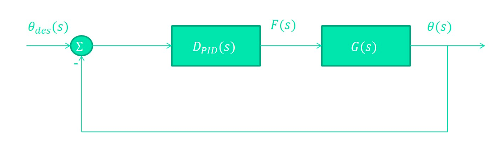
\includegraphics[scale=0.7]{Block Diagram of Controlled Pendulum}
    \caption{ Block Diagram of the Controlled Pendulum}
\end{figure} 

\begin{figure}[!htb]
    \centering
    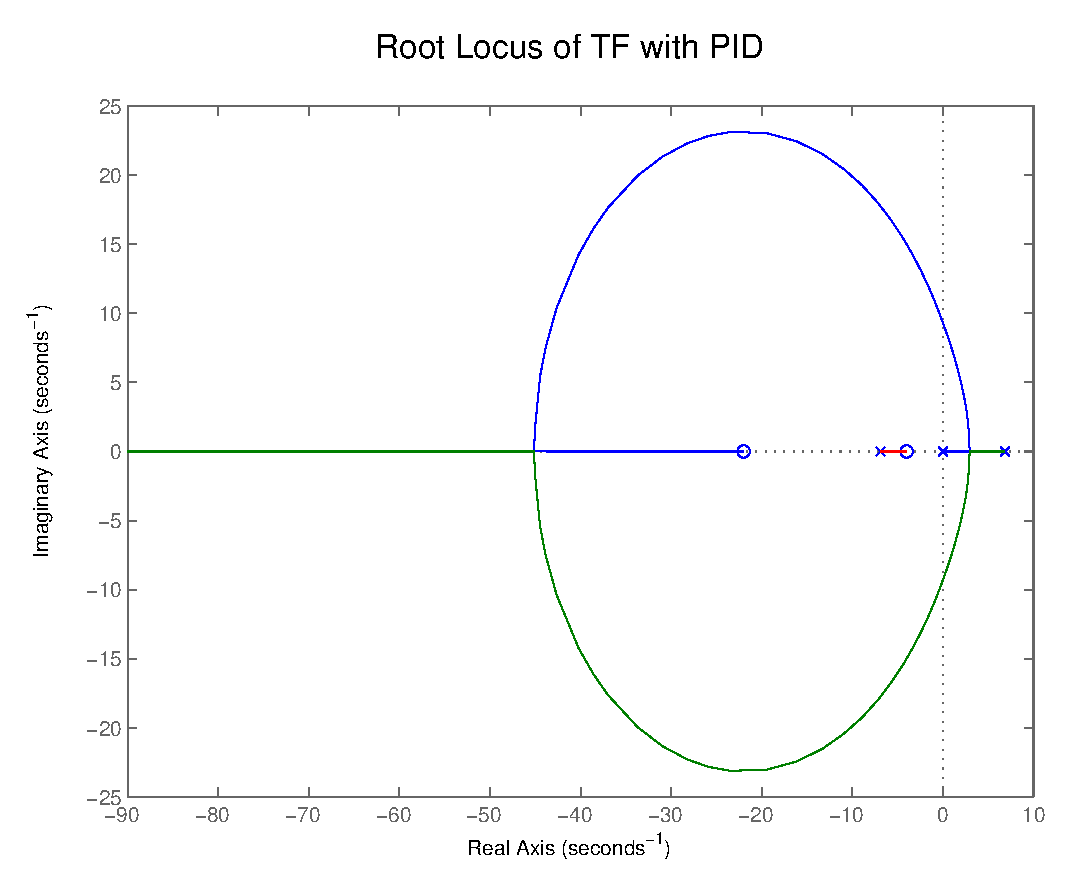
\includegraphics[scale=0.6]{1}
    \caption{ Rlocus of TF with PID Controller (varying the proportional controller)}
\end{figure} 

\begin{figure}[!htb]
    \centering
    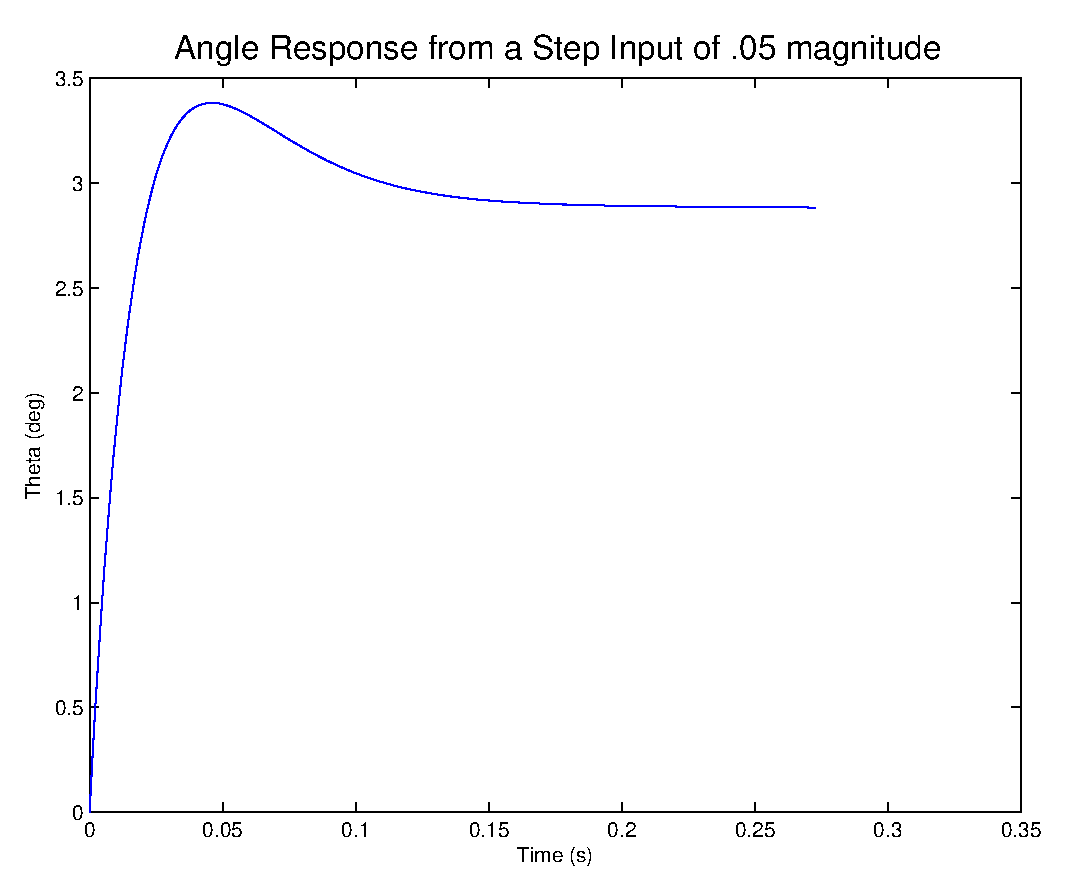
\includegraphics[scale=0.6]{2}
    \caption{Angle Response for a Step Input ($\theta_0$ = 0$^{\circ}$)}
\end{figure} 

\begin{figure}[!htb]
    \centering
    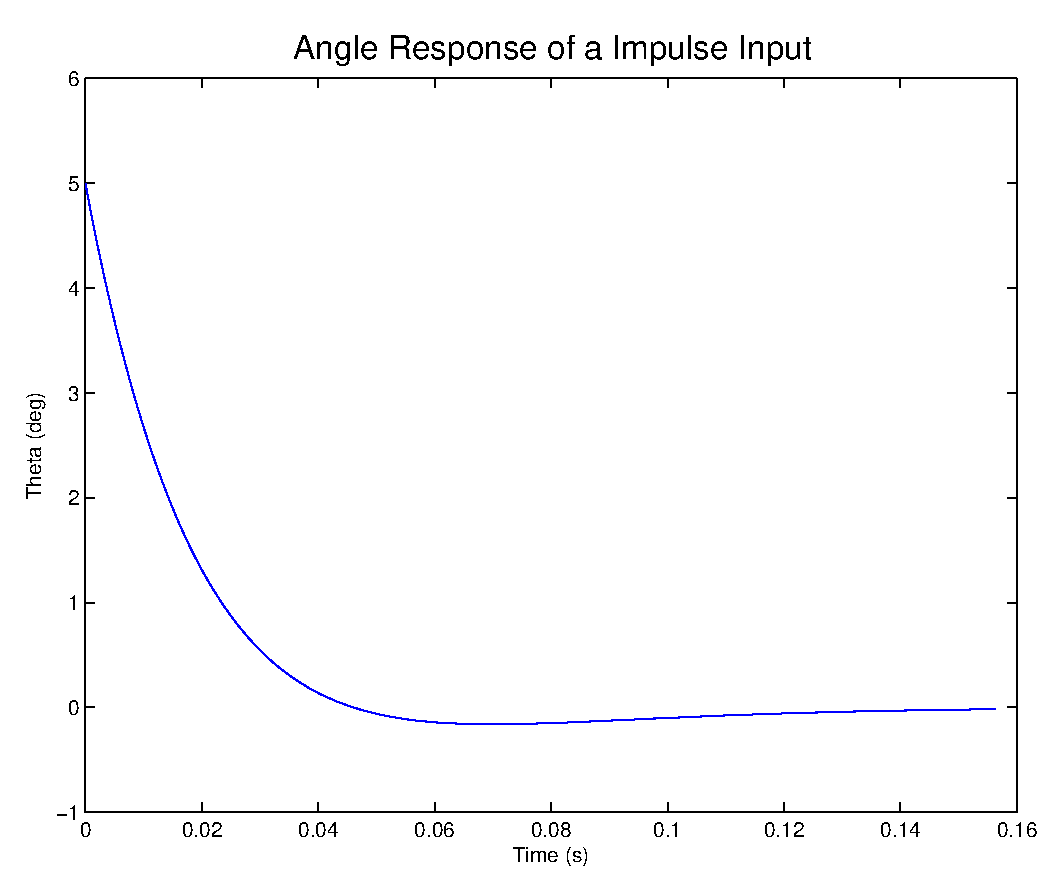
\includegraphics[scale=0.6]{3}
    \caption{Angle Response for an Impulse Input ($\theta_0$ = 5$^{\circ}$)}
\end{figure} 

\begin{figure}[!htb]
    \centering
    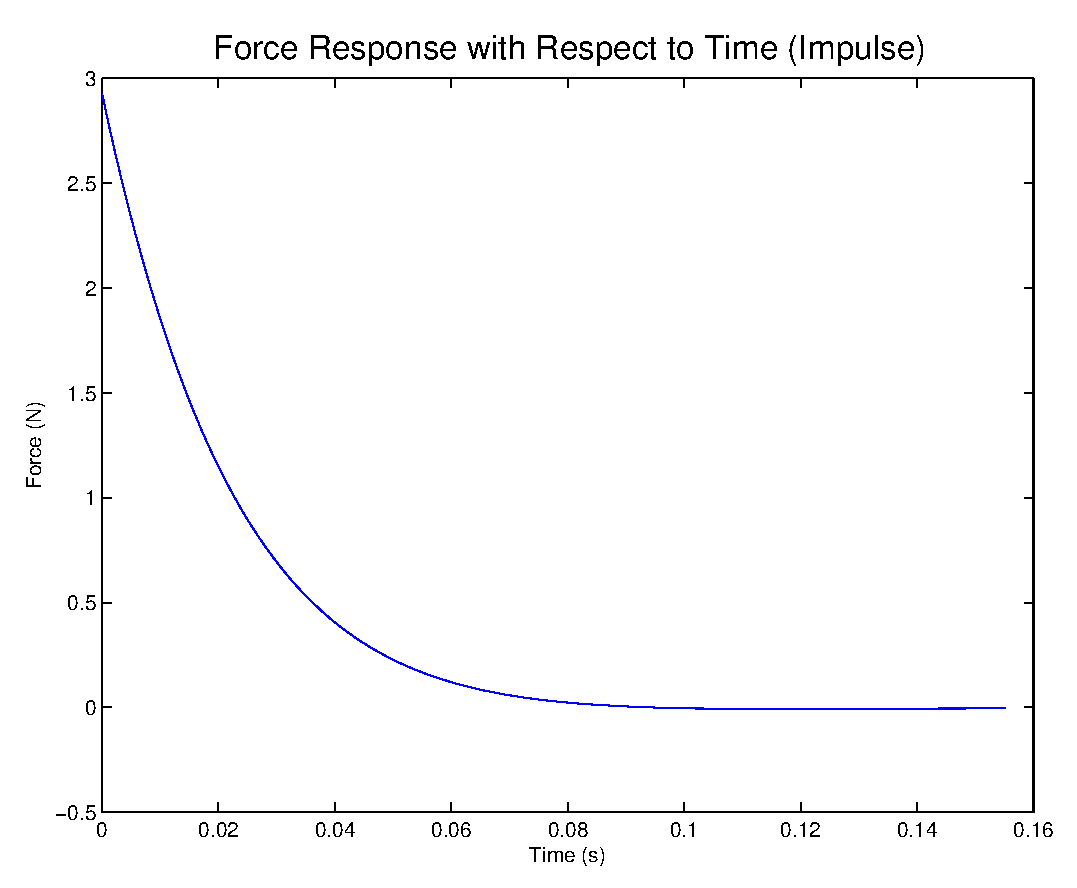
\includegraphics[scale=0.6]{4}
    \caption{Force Response of an Impulse Input ($\theta_0$ = 5$^{\circ}$)}
\end{figure} 

\begin{figure}[!htb]
    \centering
    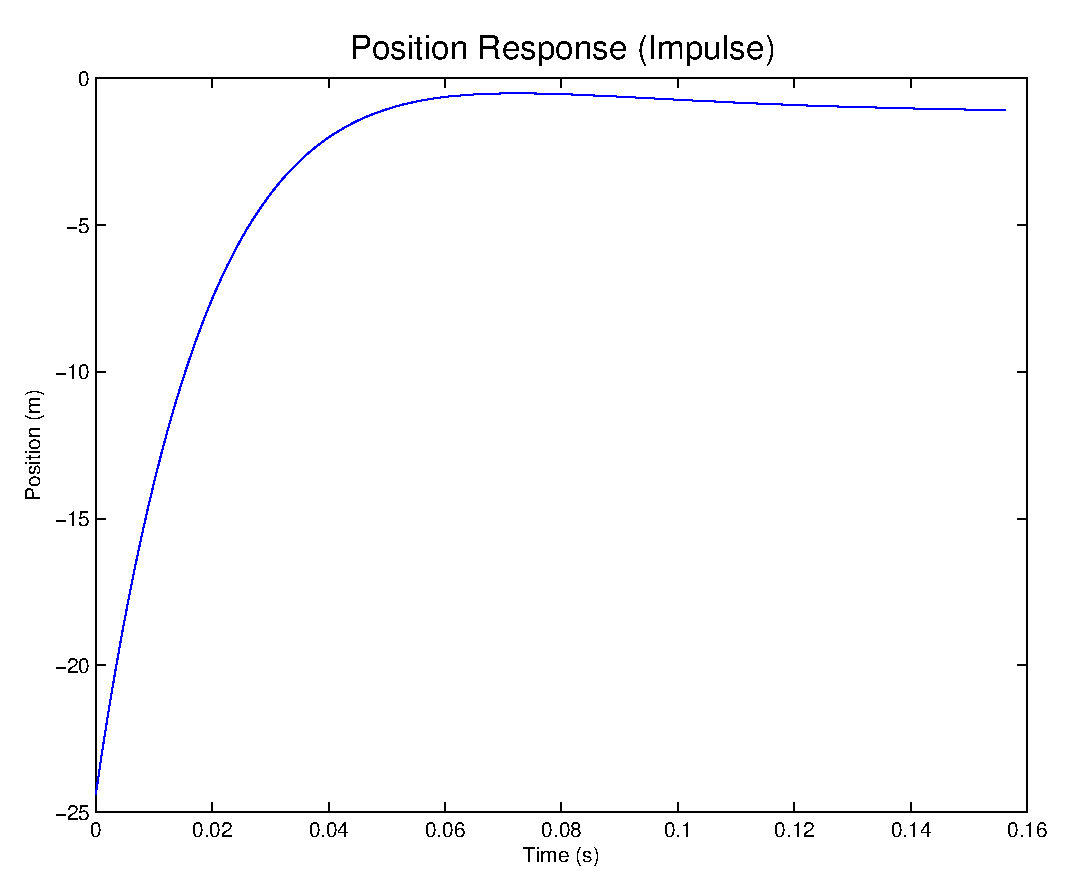
\includegraphics[scale=0.6]{5}
    \caption{Position Response of an Impulse Input ($\theta_0$ = 5$^{\circ}$)}
\end{figure} 

\begin{figure}[!htb]
    \centering
    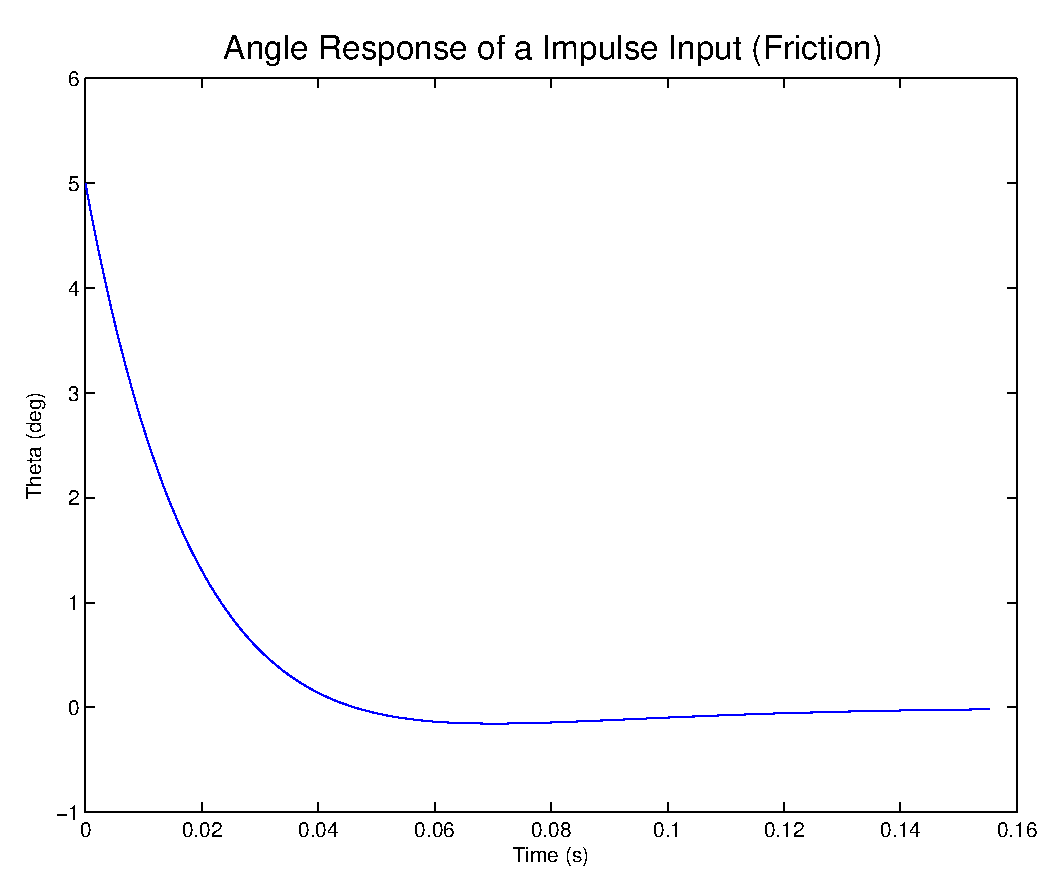
\includegraphics[scale=0.6]{6}
    \caption{Angle Response of an Impulse Input with Friction ($\theta_0$ = 5$^{\circ}$)}
\end{figure} 

\begin{figure}[!htb]
    \centering
    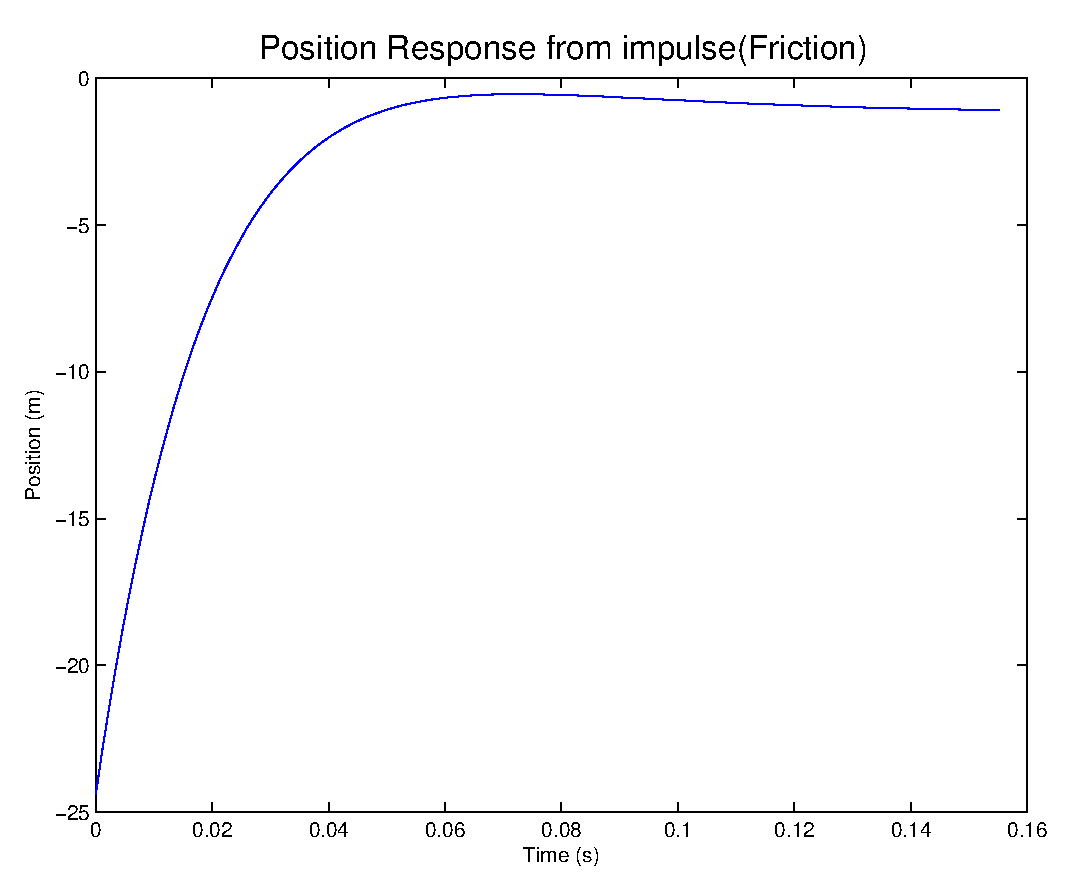
\includegraphics[scale=0.6]{7}
    \caption{Position Response of an Impulse Input with Friction ($\theta_0$ = 5$^{\circ}$)}
\end{figure} 

\FloatBarrier

\subsection{Discussion}

\subsubsection{Requirements}

My controller is stable, has 0\% steady state error for step inputs, a settling time that is .292s of the maximum, an overshoot that is 51.4\% of the maximum, and a force that is 97.7\% below the maximum. All of these values are quite satisfying except for the force that is used. I think that if I had more time, I could adjust the poles for a better value. Note that a step input is impractical for the angle because we want it to be straight up. An impulse force is much more practical for the real world.

\begin{center}
\begin{tabular}{|c | c | c|} 
\hline
 & Goal & Actual \\ 
\hline
Stability &  Stable & Stable \\ 
\hline
Steady State Error (step input)  & 0\% & 0\% \\ 
\hline
Settling Time (Max) & .5 s & .146 s \\
\hline
Overshoot (Max)& 35\% & 18.1\% \\
\hline
Force (Max) & 3N & 2.929N \\
\hline
\end{tabular}
\end{center}

\subsubsection{Friction}

Accounting for friction kept all my parameters the same or improved them except for the force used. This makes sense because it would take a larger force to overcome friction and move the pendulum the same distance. I am unsure of why the settling time and overshoot improved, my guess is that it is because the friction slows down the cart so that it the overshoot is less and the settling time improves because of this. The position response seems to be the same whether friction is accounted for or not. This is interesting because I thought that friction would slow down the cart until it stopped, but it keeps moving as long as the simulation runs. My current theory on this is that the model controls the position, so even if friction is added, the model is going to add more force to overcome the friction.

\begin{center}
\begin{tabular}{|c | c | c | c|} 
\hline
 & Goal & Actual & Actual (With Friction)\\ 
\hline
Stability &  Stable & Stable & Stable\\ 
\hline
Steady State Error (step input)  & 0\% & 0\% & 0\%\\ 
\hline
Settling Time (Max) & .5 s & .146 s & .143 s \\
\hline
Overshoot (Max)& 35\% & 18.1\% & 17.3\% \\
\hline
Force (Max) & 3N & 2.929N & 2.97N\\
\hline
\end{tabular}
\end{center}

\section{LQR State Space Controller}
\subsection{4th Order}
\subsubsection{State-Space Modeling}
Figure \ref{fig:4thOrder} shows the free-body diagrams of the inverted pendulum, cart, and motor.

\begin{figure}[!htb]
\centering
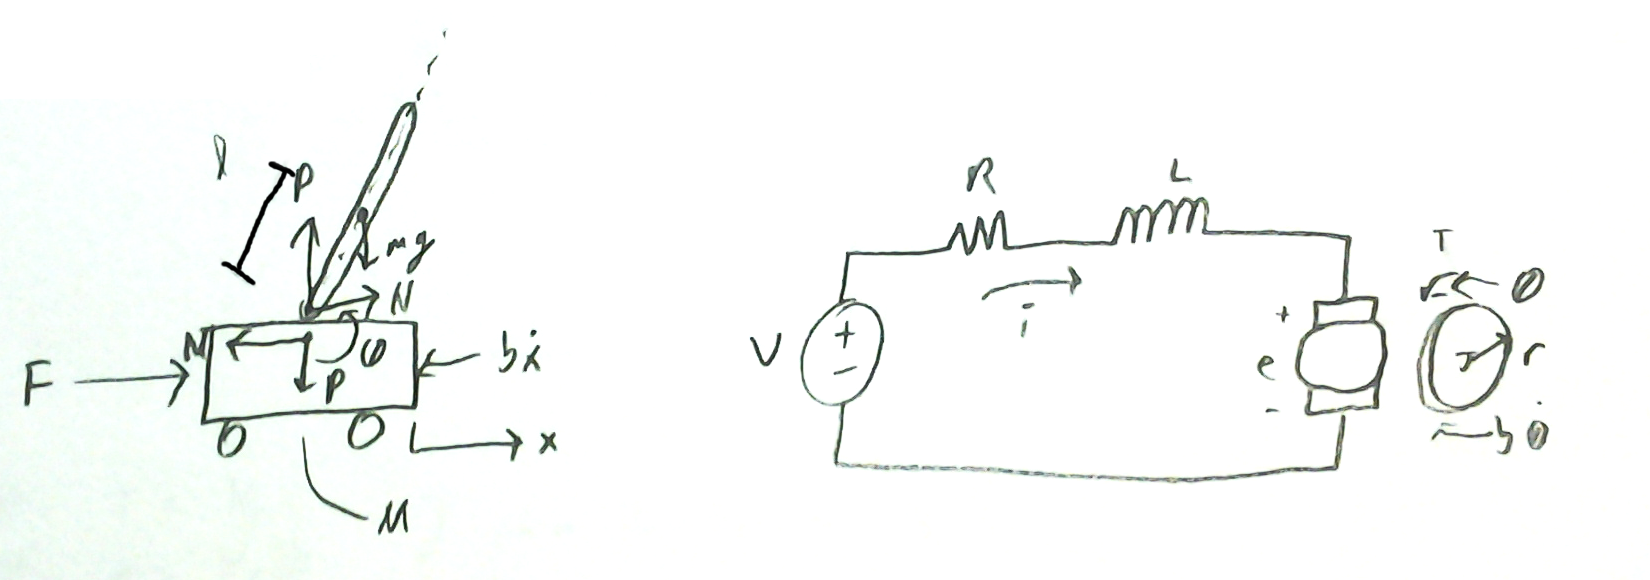
\includegraphics[width=0.95\linewidth]{System4thOrder}
\caption{4th Order System}
\label{fig:4thOrder}
\end{figure}

Summation of carts forces in the horizontal direction:
\begin{equation} 
\label{eqn1}
F = M\ddot{x}+b\dot{x} + N
\end{equation}

Summation of the pendulum forces in the horizontal direction:
\begin{equation} 
\label{eqn2}
N = m\ddot{x}+m l \ddot{\phi} cos(\phi)-m l \dot{\phi}^2sin(\phi)
\end{equation}

Substituting \ref{eqn2} into \ref{eqn1}:
\begin{equation} 
\label{eqn3}
F = M\ddot{x}+b\dot{x} + m\ddot{x}+m l \ddot{\phi} cos(\phi)-m l \dot{\phi}^2sin(\phi)
\end{equation}

Next, the sum of forces perpendicular to the pendulum
\begin{equation} 
\label{eqn4}
Psin(\phi)+Ncos(\phi)-mgsin(\phi) = m l \ddot{\phi} + m\ddot(x)cos(\phi)
\end{equation}

Summing the moments about the centroid of the pendulum
\begin{equation} 
\label{eqn5}
-P sin(\phi)-N cos(\phi) = I \ddot{\phi}/l
\end{equation}

Combining \ref{eqn4} and \ref{eqn5} leads to 
\begin{equation} 
\label{eqn6}
(I+m l^2)\ddot{\phi} + m g lsin(\phi) = -m l \ddot{x} cos(\phi)
\end{equation}

Small angle approximations. $\theta$ replaces $\phi$ so that the angle $\theta$ = 0 $\degree$ is straight up.
\\

\begin{equation} 
\label{sa1}
cos(\phi) = cos(\pi + \theta) \approx -1
\end{equation}

\begin{equation} 
\label{sa2}
sin(\phi) = sin(\pi + \theta) \approx -\theta
\end{equation}

\begin{equation} 
\label{sa3}
\dot{\phi} = \dot{\theta} \approx 0
\end{equation}

Plugging \ref{sa1} and \ref{sa2} into \ref{eqn3} and \ref{eqn6} leads to
\begin{equation} 
\label{eqn3b}
F = (M+m)\ddot{x}+b\dot{x} -m l \ddot{\theta}
\end{equation}

\begin{equation} 
\label{eqn6b}
(I+m l^2)\ddot{\theta} - m g l\theta = m l \ddot{x}
\end{equation}

Motor Equations:
\begin{equation} 
\label{eqn7}
L i + R i = V - K_m\dot{\theta_m}
\end{equation}

\begin{equation} 
\label{eqn8}
T = K_m*i
\end{equation}
\begin{equation}
F = T/r
\label{eqn:4thF}
\end{equation}

Solving equation \ref{eqn7} for $i$ after setting $L = 0$, then plugging this into equation \ref{eqn8} and then into \ref{eqn:4thF}, we get:
%F = \frac{R K_m}{r(V-K_m\dot{\theta_m})}
\begin{equation}
\label{eqn9}
F = \frac{K_m(V - K_m\dot{\theta_m})}{r R}
\end{equation}

To relate $\theta_m$ and $x$, we can say:

\begin{equation}
x = \theta_m r
\label{eqn:4thx}
\end{equation}

Plugging equation \ref{eqn:4thx} into \ref{eqn9}:

\begin{equation}
F = \frac{K_m}{r R} V - \frac{K_m^2}{r^2 R} \dot{x}
\label{eqn:4thFFinal}
\end{equation}

Finally, plugging \ref{eqn:4thFFinal} into \ref{eqn3b} and \ref{eqn6b} and solving for $\ddot{x}$ and $\ddot{\theta}$ leads to the state space equations below

\begin{equation}
\label{ss1}
\begin{bmatrix}
\dot{x}\\
\ddot{x}\\
\dot{\theta}\\
\ddot{\theta}\\
\end{bmatrix} =
\begin{bmatrix}
0&1&0&0\\
0&\frac{(I+m l^2)/(m l) (-(b+K^2/(R r^2))}{(M+m) (I+m l^2)/(m l)-m l}&\frac{(I+m l^2)/(m l) (M+m) g}{[(M+m) 		(I+m l^2)/(m l)-m l]-g}&0\\
0&0&0&1\\
0&\frac{-(b+K^2/(R r^2))}{(M+m) (I+m l^2)/(m l)-m l}&\frac{(M+m) g}{(M+m) (I+m l^2)/(m l)-m l}&0\\
\end{bmatrix}
\begin{bmatrix}
x\\
\dot{x}\\
\theta\\
\dot{\theta}\\
\end{bmatrix} +
 	\begin{bmatrix}
0\\
\frac{(I+m*l^2)/(m*l)*(K/(R*r)}{(M+m) (I+m l^2)/(m l)-m l}\\
0\\
\frac{K/(R*r)}{(M+m) (I+m l^2)/(m l)-m l}\\
\end{bmatrix} v
\end{equation}
  
\begin{equation}
\label{ss2}
\begin{bmatrix}
x\\
\theta \\
\end{bmatrix} =
\begin{bmatrix}
1&0&0&0\\
0&0&1&0\\
\end{bmatrix}
\begin{bmatrix}
x\\
\dot{x}\\
\theta\\
\dot{\theta}\\
\end{bmatrix}
\end{equation}

\subsubsection{Poles, Stability, and Observability}
Now that the state-space equations are found, the poles of the model are equal to the eigenvalues of the $A$ matrix. The original Poles are shown below:
\begin{enumerate}
  \item   0.00000 + 0.00000i
  \item -9.9916 + 0.00000i
  \item -4.9981 + 0.00000i
  \item 5.1345 + 0.00000i
\end{enumerate}
Because one of the poles is positive, the system is unstable. We will fix this with a controlled matrix $A$ in the next section.

If the rank of the controllability matrix shown below equals the number of states ($n$) the system is made up of, then the system is controllable. In our case the rank of $R$ equals 4 so our system is controllable. This means that with our controller, we can make the system reach any state.

\begin{equation} 
\label{ctrb}
\centering
R = \begin{bmatrix}
	B&AB&\hdots&A^{n-1}B\\
	\end{bmatrix}
\end{equation}
 
 If the rank of the observability matrix shown below equals the number of states the system is made up of, then the system is observable. In our case the rank of $O$ equals 4 so our system is observable. This means that in any possible situation, the current state of our system can be determined using only the inputs and outputs.
 
 \begin{equation} 
\label{obsv}
\centering
O = \begin{bmatrix}
	C\\
	CA\\
	\vdots\\
	CA^{n-1}\\
	\end{bmatrix}
\end{equation}

\subsubsection{LQR Controller}
A linear-quadratic regulator (LQR) weights factors depending on their importance using the $n$x$n$ $Q$ matrix, while minimizing another factor using the variable $R$. According to \href{http://ctms.engin.umich.edu/CTMS/index.php?example=InvertedPendulum&section=ControlStateSpace}{Inverted Pendulum: State-Space Methods for Controller Design}, a good starting point is $Q$ = $C$'$C$ and $R = 1$. In this case, because of our $C$ matrix, we will be weighting two factors: the position of the cart ($x$) and the angle of the pendulum ($\theta$). However, we care much more about the pendulum staying vertical than we do the position staying at 0 m. Because of this, after some tests we weighted $x$ at $1000$ and $\theta$ at $100,000$, giving us the $Q$ matrix below. To allow the force exerted on the cart to be greater, we decreased $R$ to be $0.1$.

 \begin{equation} 
\label{q}
\centering
Q = \begin{bmatrix}
	1000&0&0&0\\
	0&0&0&0\\
	0&0&100,000&0\\
	0&0&0&0\\
	\end{bmatrix}
\end{equation}

We could also have experimented more with the $Q$ matrix, maybe starting out with $I_4$ rather than $C$'$C$, weighting all of our states rather than just 2 of them and then adjusting all 4 of these weightings. This is future work that could be done.

In LQR controllers, the state-feedback control gains vector $k$ is used to move the poles in the system. It can be calculated by minimizing the cost function $J$. We used Octave's LQR function to calculate our $k$ vector. Once calculated, the corrected $A$ matrix $A_c$ can be calculated:

\begin{equation}
\label{ac}
A_c=[A-Bk]
\end{equation}

\subsubsection{Precompensator}
At this point, with a reference input commanding the pendulum to a certain position, the cart would move somewhere, but not to the desired position. Because of this, we had to add a precompensator to account for this error in position. We chose the C matrix below so that we would be controlling the position with our reference input:
\\

\begin{equation}
\label{pcomp}
\centering
C_n = \begin{bmatrix}
1 & 0 & 0 & 0
\end{bmatrix}
\end{equation}
 
By replacing the state space $C$ matrix with $C_n$, $\bar{N}$ can be calculated. We used the \textit{rscale} function provided by \href{http://ctms.engin.umich.edu/CTMS/index.php?aux=Extras_rscale}{Control Tutorials for Matlab \& Simulink} to calculate $\bar{N}$. $\bar{N}$ is a scale factor that eliminates the steady-state error of a system to a step input. It should be noted that $\bar{N}$ only works for single input systems, which is why we could use it to only eliminate the steady state error in the carts position. Once $\bar{N}$ is calculated, the state-space equation uses the corrected A matrix, B $\bar{N}$, C, and D for the A, B, C, and D matrices respectively.
 
 \subsubsection{Adding an Observer-Based Estimator}
 Previous work assumes full-state feedback, which means that x, $\dot{x}$, $\theta$, and $\dot{\theta}$ are all being measure. However, only x and $\theta$ are being measured so we must add observer based control. Figure \ref{fig:bd} is the previous block diagram, and Figure \ref{fig:bd2} is the updated block diagram with the observer-based estimator.

\begin{figure}
\begin{minipage}[c]{0.45\textwidth}
\centering
\subfloat[Without Observer]{{
	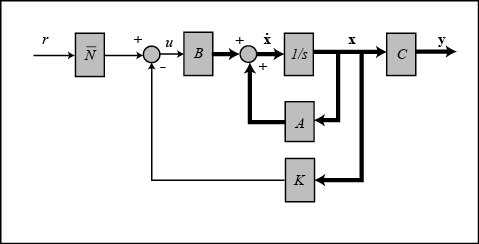
\includegraphics[width=1.0\linewidth]{blockd}
	\label{fig:bd}
}}
\end{minipage}
\begin{minipage}[c]{0.45\textwidth}
\subfloat[With Observer]{{
	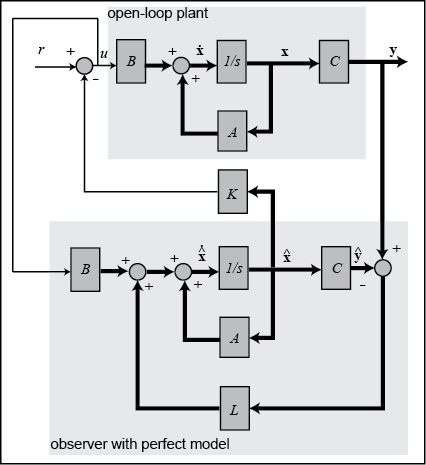
\includegraphics[width=1.0\linewidth]{observer_blockd}
	\label{fig:bd2}
}}
\end{minipage}
\caption{Adding the observer, \\ Source: \href{http://ctms.engin.umich.edu/CTMS/index.php?example=InvertedPendulum&section=ControlStateSpace}{Inverted Pendulum: State-Space Methods for Controller Design}}
\end{figure}

The speed of convergence depends on the poles of the estimator. Since we are going to use the estimation before the actual event occurs, we want the estimation to converge must faster. Because of this we want the poles of our estimator to be at least four times faster than the slowest controller pole. If the estimator poles are too fast it can cause error in the measurement, so usually the poles of the estimator should not be more than 10 times larger than the smallest controller pole. Also, the estimator poles should be close together. The current poles of our C matrix are listed below. Placing the estimator poles P at [-30, -31, -32, -33] was found to work after several trials. Note: we did not place all the estimator poles in the same position because the Octave \textit{place} function used to find L does not support that.
\begin{enumerate}
  \item  -50.8860 +50.1382i
  \item -50.8860 -50.1382i
  \item -0.7136 + 0.6863i
  \item -0.7136 - 0.6863i
\end{enumerate}

Based on the estimator poles, we used the Octave place function which computes L. Based on the Original A, B, C, and D matrices for state space, the final state space equations are shown below:

\begin{equation}
\label{ss3}
\begin{bmatrix}
\dot{x}\\
\dot{e}\\
\end{bmatrix}
=
\begin{bmatrix}
A-Bk&Bk\\
0&A-LC\\
\end{bmatrix}
\begin{bmatrix}
x\\
e\\
\end{bmatrix} +
\begin{bmatrix}
B\bar{N}\\
0\\
\end{bmatrix} r
\end{equation}

\begin{equation}
\label{ss4}
y = 
\begin{bmatrix}
C&0\\
\end{bmatrix}
\begin{bmatrix}
X\\
e\\
\end{bmatrix} +
\begin{bmatrix}
0\\
\end{bmatrix} r
\end{equation}

Then, to allow us to use this observer when actually using the pendulum, we needed to derive a non-closed-loop continuous state-space model that we could discretize and then run iteratively at our sample rate. By coming up with new A, B, C, and D matrices, we used the \textit{c2d} command in Octave to do this.

\begin{equation*}
\dot{\hat{x}} = A \hat{x} + B u + L(y - \hat{y})
\end{equation*}
\begin{equation*}
y = C \hat{x} + D u
\end{equation*}
\begin{equation*}
\implies \dot{\hat{x}} = A \hat{x} + \begin{bmatrix}
B & L
\end{bmatrix} \begin{bmatrix}
u \\
y - \hat{y}
\end{bmatrix}
\end{equation*}
\begin{equation*}
y = C \hat{x} + \begin{bmatrix}
D & 0 & 0
\end{bmatrix} \begin{bmatrix}
u \\
y - \hat{y}
\end{bmatrix}
\end{equation*}

This state space model successfully keeps the pendulum up and the cart centered on the track. However, there is some noise which is not accounted for that causes the pendulum to oscillate more than it should. Also, originally this model only works with the wrong radius value for the motor which we used from a previous model that worked. However, after measuring the PWM input provided to the motor, we discovered the signal ranged from -30V to 30V instead of -20V to 20V like we were told. Once we made this change, the inverted pendulum worked with the correct radius.

\subsection{8th Order}
\begin{figure}[!htb]
\centering
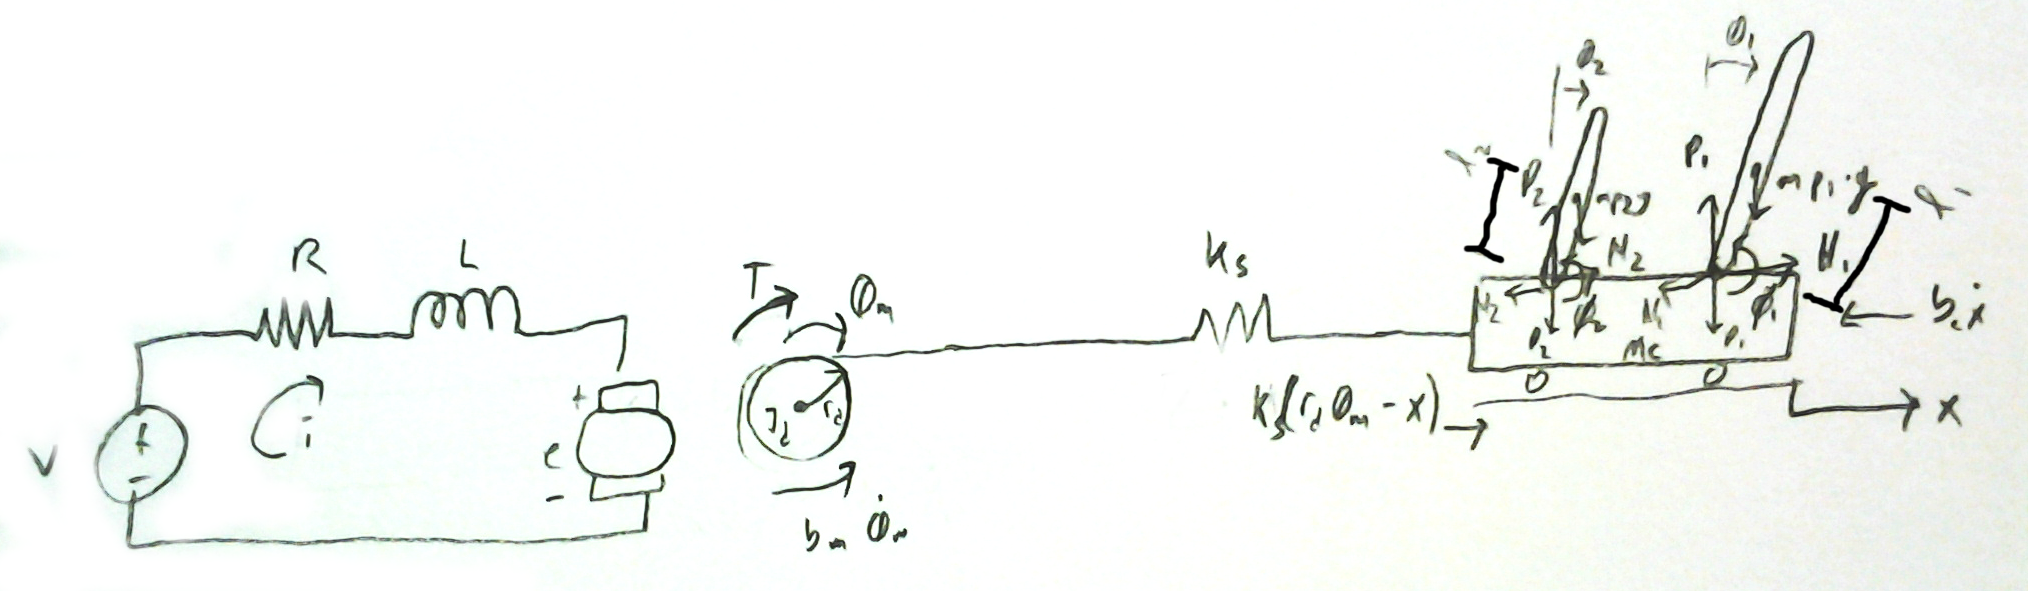
\includegraphics[width=0.95\linewidth]{System8thOrder}
\caption{8th Order System. Note the changes in notation from the 4th order model to more closely match the parameters in our Octave script. There's so many parameters we didn't want to make a mistake when entering our equations into Octave.}
\label{fig:8thOrder}
\end{figure}

We derived 8th order equations which include the springiness of the wire which moves the cart only to discover that the matrix had a rank of 7 meaning that the state space equations were not controllable. This is because when modeling the movement of the wire as a spring, the position of the cart is not known. This system is shown in Figure \ref{fig:8thOrder}.

We started off with the motor equations:
\begin{equation}
J_d \ddot{\theta}_m + b_m \dot{\theta}_m = K_m i
\label{eqn:8th1}
\end{equation}
\begin{equation}
L \dot{i} + R i = V - K_m \dot{\theta}_m
\label{eqn:8th2}
\end{equation}
\begin{equation}
T = K_m i
\label{eqn:8th3}
\end{equation}

Equation for the cart:
\begin{equation*}
\rightarrow \sum{F} = m a
\end{equation*}
\begin{equation*}
\implies -b_c \dot{x} - N_1 - N_2 + K_s (r_d \theta_m - x) = M_c \ddot{x}
\end{equation*}

\begin{equation}
\implies M_c \ddot{x} + b_c \dot{x} + K_s x - K_s r_d \theta_m + N_1 + N_2 = 0
\label{eqn:8th4}
\end{equation}

For each pendulum:
\begin{equation*}
\rightarrow \sum{F} = ma
\end{equation*}
\begin{equation}
\implies N_1 = m_{p1} \ddot{x} + m_{p1} l_1 \ddot{\phi}_1 cos(\phi_1) - m_{p1} l_1 \dot{\phi}_1^2 sin(\phi_1)
\label{eqn:8th5}
\end{equation}
and \begin{equation}
\implies N_2 = m_{p2} \ddot{x} + m_{p2} l_2 \ddot{\phi}_2 cos(\phi_2) - m_{p2} l_2 \dot{\phi}_2^2 sin(\phi_2)
\label{eqn:8th6}
\end{equation}

Plugging equation \ref{eqn:8th5} and \ref{eqn:8th6} into \ref{eqn:8th4}, where $F = K_s ( r_d \theta_m - x )$:
\begin{equation*}
\begin{split}
M_c \ddot{x} + b_c \dot{x} + m_{p1} \ddot{x} + m_{p1} l_1 \ddot{\phi}_1 cos(\phi_1) - m_{p1} l_1 \dot{\phi}_1^2 sin(\phi_1) + \\
m_{p2} \ddot{x} + m_{p2} l_2 \ddot{\phi}_2 cos(\phi_2) - m_{p2} l_2 \dot{\phi}_2^2 sin(\phi_2) = F
\end{split}
\end{equation*}

\begin{equation}
\begin{split}
\implies (M_c + m_{p1} + m_{p2}) \ddot{x} + b_c \dot{x} + m_{p1} l_1 \ddot{\phi}_1 cos(\phi_1) - m_{p1} l_1 \dot{\phi}_1^2 sin(\phi_1) + \\
m_{p2} l_2 \ddot{\phi}_2 cos(\phi_2) - m_{p2} l_2 \dot{\phi}_2^2 sin(\phi_2) = F
\end{split}
\label{eqn:8th7}
\end{equation}

For each pendulum,
\begin{equation}
P_1 sin(\phi_1) + N_1 cos(\phi_1) - m_{p1} g sin(\phi_1) = m_{p1} l_1 \ddot{\phi}_1 + m_{p1} \ddot{x} cos(\phi_1)
\label{eqn:8th8}
\end{equation}

\begin{equation}
P_2 sin(\phi_2) + N_2 cos(\phi_2) - m_{p2} g sin(\phi_2) = m_{p2} l_2 \ddot{\phi}_2 + m_{p2} \ddot{x} cos(\phi_2)
\label{eqn:8th9}
\end{equation}

and moments:
\begin{equation}
-P_1 l_1 sin(\phi_1) - N_1 l_1 cos(\phi_1) = J_1 \ddot{\phi}_1
\label{eqn:8th10}
\end{equation}
%\begin{equation*}
%\implies -l_1 ( P_1 sin(\phi_1) + N_1 cos(\phi_1) = J_1 \ddot{\phi}_1
%\end{equation*}
%\begin{equation*}
%\implies P_1 sin(\phi_1) + N_1 cos(\phi_1) = - (J_1/l_1) \ddot{\phi}_1
%\end{equation*}

\begin{equation}
-P_2 l_2 sin(\phi_2) - N_2 l_2 cos(\phi_2) = J_2 \ddot{\phi}_2
\label{eqn:8th11}
\end{equation}
%\begin{equation*}
%\implies -l_2 ( P_2 sin(\phi_2) + N_2 cos(\phi_2) = J_2 \ddot{\phi}_2
%\end{equation*}
%\begin{equation*}
%\implies P_2 sin(\phi_2) + N_2 cos(\phi_2) = - (J_2/l_2) \ddot{\phi}_2
%\end{equation*}

Plugging equation \ref{eqn:8th10} into \ref{eqn:8th8}, we get:
\begin{equation*}
\implies - (J_1 / l_1) \ddot{\phi}_1 - m_{p1} g sin(\phi_1) = m_{p1} l_1 \ddot{\phi}_1 + m_{p1} \ddot{x} cos(\phi_1)
\end{equation*}
\begin{equation*}
\implies (m_{p1} l_1 + (J_1 / l_1)) \ddot{\phi}_1 + m_{p1} g sin(\phi_1) = -m_{p1} \ddot{x} cos(\phi_1)
\end{equation*}
\begin{equation}
\implies (m_{p1} l_1^2 + J_1) \ddot{\phi}_1 + m_{p1} g l_1 sin(\phi_1) = -m_{p1} l_1 \ddot{x} cos(\phi_1)
\label{eqn:8th12}
\end{equation}

And, similarly, plugging \ref{eqn:8th11} into \ref{eqn:8th9}, we get:
\begin{equation}
\implies (m_{p2} l_2^2 + J_2) \ddot{\phi}_2 + m_{p2} g l_2 sin(\phi_2) = -m_{p2} l_2 \ddot{x} cos(\phi_2)
\label{eqn:8th13}
\end{equation}

Applying small angle approximations, where $\phi_1 = \pi + \theta_1$, first for the long pendulum, where we want it to stay up:
\begin{equation*}
cos(\phi_1) = cos(\pi + \theta_1) \approx -1
\end{equation*}
\begin{equation*}
sin(\phi_1) = sin(\pi + \theta_1) \approx - \theta_1
\end{equation*}
\begin{equation*}
\dot{\phi}_1^2 = \dot{\theta}_1^2 \approx 0
\end{equation*}

And then for the short pendulum, where $\phi_2 = \theta_2$, since we want it to hang down:
\begin{equation*}
cos(\phi_2) = cos(\theta_2) \approx 1 - \theta_2^2 / 2 \approx 1
\end{equation*}
\begin{equation*}
sin(\phi_2) = sin(\theta_2) \approx \theta_2
\end{equation*}
\begin{equation*}
\dot{\phi}_2^2 = \dot{\theta}_2^2 \approx 0
\end{equation*}

Plugging all of these small angle approximations into equations \ref{eqn:8th12}, \ref{eqn:8th13}, and \ref{eqn:8th7}:
\begin{equation*}
(m_{p1} l_1^2 + J_1) \ddot{\theta}_1 + m_{p1} g l_1 (-\theta_1) = -m_{p1} l_1 \ddot{x} (-1)
\end{equation*}
\begin{equation}
\implies (m_{p1} l_1^2 + J_1) \ddot{\theta}_1 - m_{p1} g l_1 \theta_1 = m_{p1} l_1 \ddot{x}
\label{eqn:8th14}
\end{equation}

\begin{equation*}
(m_{p2} l_2^2 + J_2) \ddot{\theta}_2 + m_{p2} g l_2 (-\theta_2) = -m_{p2} l_2 \ddot{x} (-1)
\end{equation*}
\begin{equation}
\implies (m_{p2} l_2^2 + J_2) \ddot{\theta}_2 - m_{p2} g l_2 \theta_2 = m_{p2} l_2 \ddot{x}
\label{eqn:8th15}
\end{equation}

\begin{equation}
(M_c + m_{p1} + m_{p2}) \ddot{x} + b_c \dot{x} - m_{p1} l_1 \ddot{\theta}_1 + m_{p2} l_2 \ddot{\theta}_2 = F
\label{eqn:8th16}
\end{equation}

If $L = 0$ in equations \ref{eqn:8th1}, \ref{eqn:8th2}, and \ref{eqn:8th3}, then:
\begin{equation*}
J_d \ddot{\theta}_m + b_m \dot{\theta}_m = K_m i
\end{equation*}
\begin{equation*}
R i = V - K_m \dot{\theta}_m
\end{equation*}
\begin{equation}
\implies i = (1/R) V - (K_m/R) \dot{\theta}_m
\label{eqn:i}
\end{equation}
\begin{equation*}
\implies J_d \ddot{\theta}_m + b_m \dot{\theta}_m = (K_m/R) V - (K_m^2/R) \dot{\theta}_m
\end{equation*}
\begin{equation}
\implies J_d \ddot{\theta}_m + (b_m + K_m^2/R) \dot{\theta}_m - (K_m/R) V = 0
\label{eqn:8th20}
\end{equation}

Let our states be:

\begin{equation*}
\vec{x} = \begin{bmatrix}
x & \dot{x} & \theta_1 & \dot{\theta}_1 & \theta_2 & \dot{\theta}_2 & \theta_m & \dot{\theta}_m
\end{bmatrix} '
\end{equation*}

Now, using equations \ref{eqn:8th14}, \ref{eqn:8th15}, \ref{eqn:8th16}, and \ref{eqn:8th20} to solve for $\ddot{\theta}_m$, $\ddot{\theta}_1$, $\ddot{\theta}_2$, $\ddot{x}$, etc. for state space using Maple, we get the following, where $p = M_c l_1^2 l_2^2 m_{p1} m_{p2}+J_1 M_c l_2^2 m_{p2}+J_1 l_2^2 m_{p1} m_{p2}+J_2 M_c l_1^2 m_{p1}+J_2 l_1^2 m_{p1} m_{p2}+J_1 J_2 M_c+J_1 J_2 m_{p1}+J_1 J_2 m_{p2}$:

\begin{equation*}
A(:,1:4) = \begin{bmatrix}
0 & 1 & 0 & 0 \\

\begin{split}
-(-K_s l_1^2 l_2^2 m_{p1} m_{p2} \\ -J_1 K_s l_2^2 m_{p2} \\ -J_2 K_s l_1^2 m_{p1} \\ -J_1 J_2 K_s)/p
\end{split}
&
\begin{split}
-(b_c l_1^2 l_2^2 m_{p1} m_{p2} \\ +J_1 b_c l_2^2 m_{p2} \\ +J_2 b_c l_1^2 m_{p1} \\ +J_1 J_2 b_c)/p
\end{split}
&
\begin{split}
-(-g l_1^2 l_2^2 m_{p1}^2 m_{p2} \\ -J_2 g l_1^2 m_{p1}^2)/p
\end{split}
&
0 \\

0 & 0 & 0 & 1 \\

\begin{split}
-(-K_s l_2^2 m_{p2} \\ -J_2 K_s) l_1 m_{p1}/p
\end{split}
&
\begin{split}
-(b_c l_2^2 m_{p2} \\ +J_2 b_c) l_1 m_{p1}/p
\end{split}
&
\begin{split}
-(-M_c g l_2^2 m_{p2} \\ -g l_2^2 m_{p1} m_{p2} \\ -J_2 M_c g-J_2 g m_{p1} \\ -J_2 g m_{p2}) l_1 m_{p1}/p
\end{split}
&
0 \\

0 & 0 & 0 & 0 \\

\begin{split}
m_{p2} l_2 (-K_s l_1^2 m_{p1} \\ -J_1 K_s)/p
\end{split}
&
\begin{split}
m_{p2} l_2 (b_c l_1^2 m_{p1} \\ +J_1 b_c)/p
\end{split}
&
-m_{p2} l_2 g l_1^2 m_{p1}^2/p
&
0 \\

0 & 0 & 0 & 0 \\

0 & 0 & 0 & 0 \\
\end{bmatrix}
\end{equation*}

and
\begin{equation*}
A(:,5:8) = \begin{bmatrix}
0 & 0 & 0 & 0 \\

\begin{split}
-(-g l_1^2 l_2^2 m_{p1} m_{p2}^2 \\ -J_1 g l_2^2 m_{p2}^2)/p
\end{split}
&
0
&
\begin{split}
-(K_s l_1^2 l_2^2 m_{p1} m_{p2} r_d \\ +J_1 K_s l_2^2 m_{p2} r_d \\ +J_2 K_s l_1^2 m_{p1} r_d \\ +J_1 J_2 K_s r_d)/p
\end{split}
&
0 \\

0 & 0 & 0 & 0 \\

g l_2^2 m_{p2}^2 l_1 m_{p1}/p
&
0
&
\begin{split}
-(K_s l_2^2 m_{p2} r_d \\ +J_2 K_s r_d) l_1 m_{p1}/p
\end{split}
&
0 \\

0 & 1 & 0 & 0 \\

\begin{split}
m_{p2} l_2 (-M_c g l_1^2 m_{p1} \\ -g l_1^2 m_{p1} m_{p2} \\ -J_1 M_c g-J_1 g m_{p1} \\ -J_1 g m_{p2})/p
\end{split}
&
0
&
\begin{split}
m_{p2} l_2 (K_s l_1^2 m_{p1} r_d \\ +J_1 K_s r_d)/p
\end{split}
&
0 \\

0 & 0 & 0 & 1 \\

0 & 0 & 0 &
\begin{split}
-(K_m^2+ R b_m) \\ /(J_d R)
\end{split} \\
\end{bmatrix}
\end{equation*}

\begin{equation*}
B =  \begin{bmatrix}
0 & 0 & 0 & 0 & 0 & 0 & 0 & K_m/(J_d R)
\end{bmatrix} '
\end{equation*}

\begin{equation*}
C = \begin{bmatrix}
1 & 0 & 0 & 0 & 0 & 0 & 0 & 0 \\
0 & 0 & 1 & 0 & 0 & 0 & 0 & 0
\end{bmatrix}
\end{equation*}

\begin{equation*}
D = \begin{bmatrix}
0 \\
0
\end{bmatrix}
\end{equation*}

However, the rank of the controllability and observability matrices is 7, not 8. Thus this system is neither controllable nor observable, and we couldn't actually create a controller for this system.

\subsection{6th Order}
\begin{figure}[!htb]
\centering
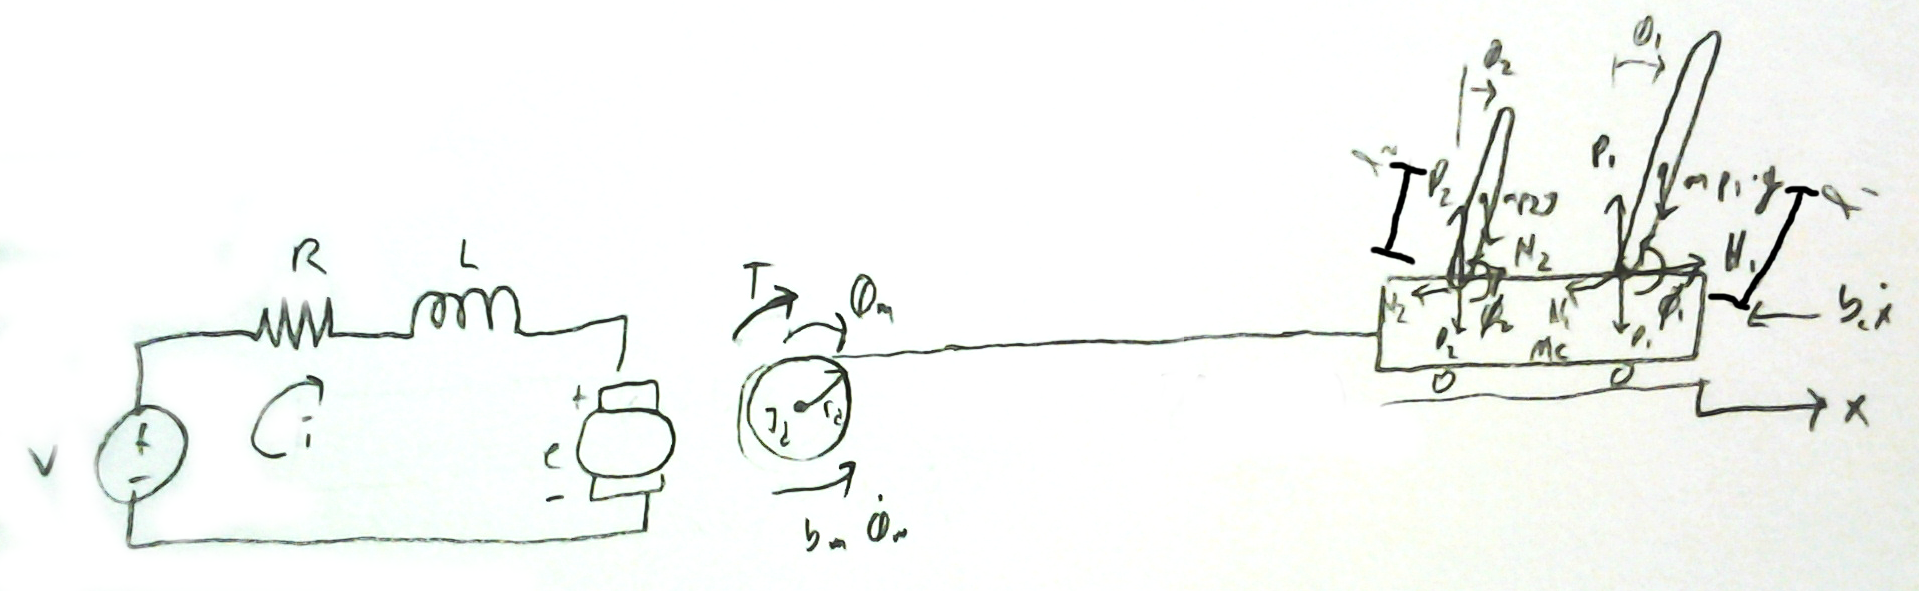
\includegraphics[width=0.95\linewidth]{System6thOrder}
\caption{6th Order System}
\label{fig:6thOrder}
\end{figure}

Since the 8th order doesn't work, we decided to go with a 6th order system that is like the 4th order system but also takes into account the short pendulum angle. We did this to see if it would eliminate some of the faulty state estimates we were having with the 4th order system, which seemed to be causing our pendulum to oscillate. Also, with only a modification to what small angle approximations we make, the equations can be used to make both pendulums stay up. The case where both pendulums are up is shown in Figure \ref{fig:6thOrder}. The only change for making the short pendulum hang down is defining $\theta_2 = \phi_2$ rather than $\theta_2 = \pi + \phi_2$. We will derive this latter case, where the short pendulum is hanging down.

Similar to equations \ref{eqn:8th14}, \ref{eqn:8th15}, and \ref{eqn:8th16}, we have:

\begin{equation} 
\label{eqn6th1}
(m_{p1} l_1^2+J_1) \ddot{\theta_1}-m_{p1} g l_1 \theta_1 = m_{p1} l_1 \ddot{x}
\end{equation}

\begin{equation} 
\label{eqn6th2}
(m_{p2} l_2^2+J_2) \ddot{\theta_2}+m_{p2} g l_2 \theta_2 = -m_{p2} l_2 \ddot{x}
\end{equation}

\begin{equation} 
\label{eqn6th3}
(M_c+m_{p1}+m_{p2}) \ddot{x}+b_c \dot{x}-m_{p1} l_1 \ddot{\theta_1}+m_{p2} l_2 \ddot{\theta_2} = F
\end{equation}

Finally, let us find the force $F$ in terms of the DC motor equations:

\begin{equation*}
F = T / r
\end{equation*}
\begin{equation*}
T = K_m i
\end{equation*}
\begin{equation*}
\implies F = (K_m / r_d) i
\end{equation*}

Then plugging in Equation \ref{eqn:i} for $i$, we get:
\begin{equation}
F = (K_m/r_d)((1/R)V - K_m/(R r_d) \dot{x}) = K_m/(R r_d) V - K_m^2 / (R r_d^2) \dot{x}
\label{eqn:F}
\end{equation}

By solving equations \ref{eqn6th1}, \ref{eqn6th2}, \ref{eqn6th3}, and \ref{eqn:F} for $\ddot{x}$, $\ddot{\theta_1}$, and $\ddot{\theta_2}$ in Maple we found:

\begin{multline} 
\label{eqn6th4}
\ddot{x} = (-(R b_c l_1^2 l_2^2 m_{p1} m_{p2} r_d^2+J_1 R b_c l_2^2 m_{p2} r_d^2+J_2 R b_c l_1^2 m_{p1} r_d^2+K_m^2 l_1^2 l_2^2*m_{p1} m_{p2}+J_1 J_2 R b_c r_d^2+\\J_1 K_m^2 l_2^2 m_{p2}+J_2 K_m^2 l_1^2 m_{p1}+J_1 J_2 K_m^2)/p_1)\dot{x} -((-R g l_1^2 l_2^2 m_{p1}^2 m_{p2} r_d^2-J_2 R g l_1^2 m_{p1}^2 r_d^2)/p_1)\theta_1 \\-((R g l_1^2 l_2^2 m_{p1} m_{p2}^2 r_d^2+J_1 R g l_2^2 m_{p2}^2 r_d^2)/p_1 \theta_2 -(-K_m l_1^2 l_2^2 m_{p1} m_{p2} r_d-J_1 K_m l_2^2 m_{p2} r_d-J_2 K_m l_1^2 m_{p1} r_d-\\J_1 J_2 K_m r_d) V/p_1
\end{multline}

\begin{multline} 
\label{eqn6th5}
\ddot{\theta_1} = -(R b_c l_2^2 m_{p2} r_d^2+J_2 R b_c r_d^2+K_m^2*l_2^2*m_{p2}+J_2*K_m^2)*l_1*m_{p1} \dot{x}/p_1 -\\(-M_c R g l_2^2 m_{p2} r_d^2-R g l_2^2 m_{p1} m_{p2} r_d^2-2 R g l_2^2 m_{p2}^2 r_d^2-J_2 M_c R g r_d^2-J_2 R g m_{p1} r_d^2-J_2 R g m_{p2} r_d^2) l_1 m_{p1} \theta_1 /p_1-\\g l_2^2 m_{p2}^2 l_1 m_{p1} \theta_2/p_1-(-K_m l_2^2 m_{p2} r_d-J_2 K_m r_d) l_1 m_{p1} V/p_1
\end{multline}

\begin{multline} 
\label{eqn6th6}
\ddot{\theta_2} = -m_{p2} l_2 (R b_c l_1^2 m_{p1} r_d^2+J_1 R b_c r_d^2+K_m^2 l_1^2 m_{p1}+J_1 K_m^2)\dot{x}/p_1 +m_{p2} l_2 g l_1^2 m{p1}^2 \theta_1/p_2 - \\m_{p2} l_2 (-M_c R g l_1^2 m_{p1} r_d^2-R g l_1^2 m_{p1} m_{p2} r_d^2-J_1 M_c R g r_d^2-J_1 R g m_{p1} r_d^2-J_1 R g m_{p2} r_d^2) \theta_2/p_1 + \\m_{p2} l_2 (-K_m l_1^2 m_{p1} r_d-J_1 K_m r_d)/p_1
\end{multline}

where 

\begin{multline} 
\label{p1}
p_1 = (R r_d^2 (M_c l_1^2 l_2^2 m_{p1} m_{p2}+2 l_1^2 l_2^2 m_{p1} m_{p2}^2+J_1 M_c l_2^2 m_{p2}+J_1 l_2^2 m_{p1} m_{p2}+\\2 J_1 l_2^2 m_{p2}^2+J_2 M_c l_1^2 m_{p1}+J_2 l_1^2 m_{p1} m_{p2}+J_1 J_2 M_c+J_1 J_2 m_{p1}+J_1 J_2 m_{p2}))
\end{multline}

and 

\begin{multline}
\label{p2}
 p_2 = (M_c l_1^2 l_2^2 m_{p1}m_{p2}+2 l_1^2 l_2^2 m_{p1} m_{p2}^2+J_1+M_c l_2^2 m_{p2}+J_1 l_2^2 m_{p1} m_{p2}+\\2 J_1 l_2^2 m_{p2}^2+J_2 M_c l_1^2 m_{p1}+J_2 l_1^2 m_{p1} m_{p2}+J_1 J_2 M_c+J_1 J_2 m_{p1}+J_1 J_2 m_{p2})
\end{multline}

We did similarly for the case where both pendulums are up. However, we will not show those equations since they resemble those above, and we put into the Octave code.

After rewriting these equations in state space form and actually running it on the pendulum, we had more oscillation than on the 4th order when using the wrong voltage and radius. We are not sure why this is -- the 6th order model should have better results than the 4th order model. Possible explanations include our 6th order model not being tuned as well as our 4th order or that there is more error in our small pendulum model than if we just ignore it. However, the oscillation decreased with this model using the correct values.

\section{Results}

Figure \ref{fig:4osrwc} and \ref{fig:6osrwc} show the step response to a reference input telling the cart to go to 0.2 meters. You will notice that it doesn't actually go to 0.2 meters. This is fixed by multiplying the reference input by $\bar{N}$. The result is Figure \ref{fig:4osrwpc} and \ref{fig:6osrwpc}, where the cart does go to a position of 0.2 meters. Also note that Figure \ref{fig:6osrwpc} has some higher frequency components that is due to it caring about the short pendulum in addition to the long pendulum.

\begin{figure}
\centering
\subfloat[4th Order]{{
	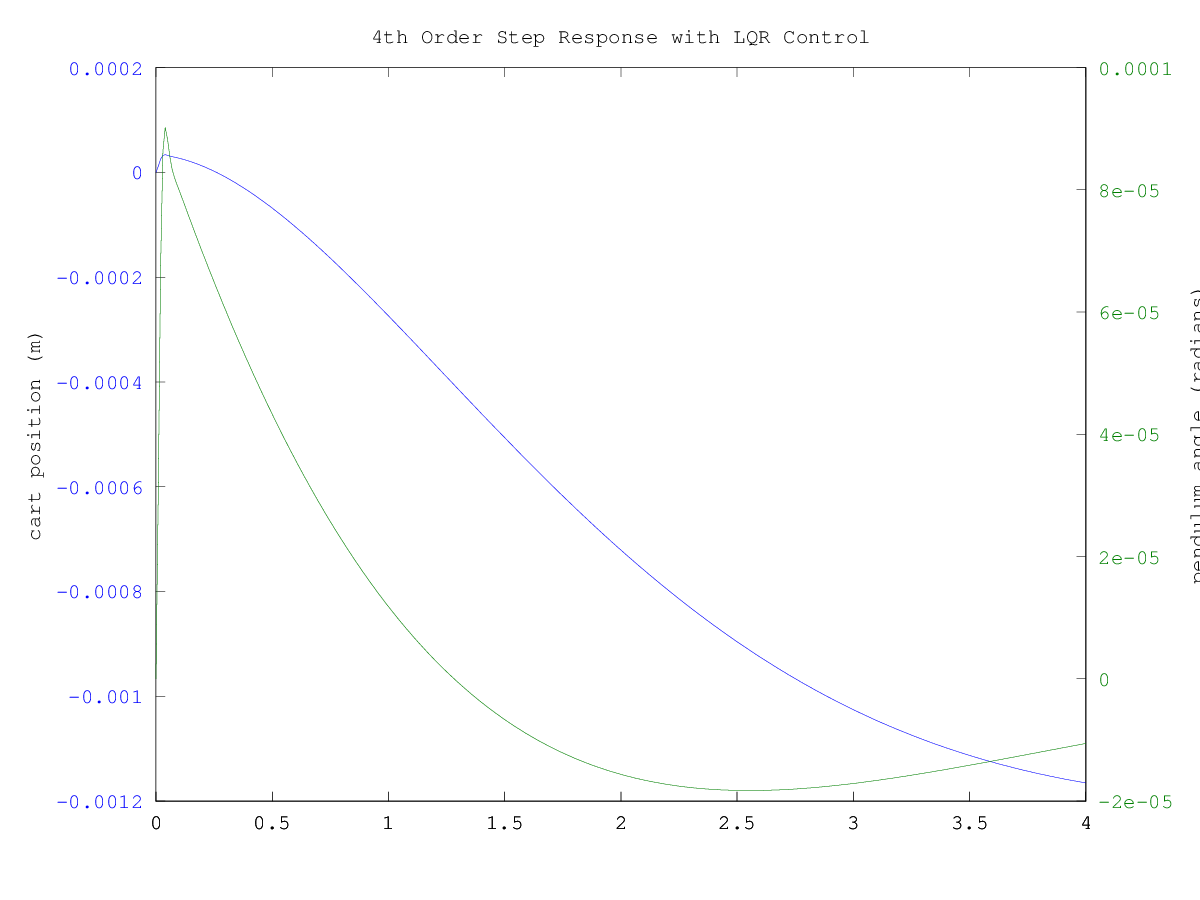
\includegraphics[width=0.5\linewidth]{4th_Order_Step_Response_with_LQR_Control}
	\label{fig:4osrwc}
}}
\subfloat[6th Order]{{
	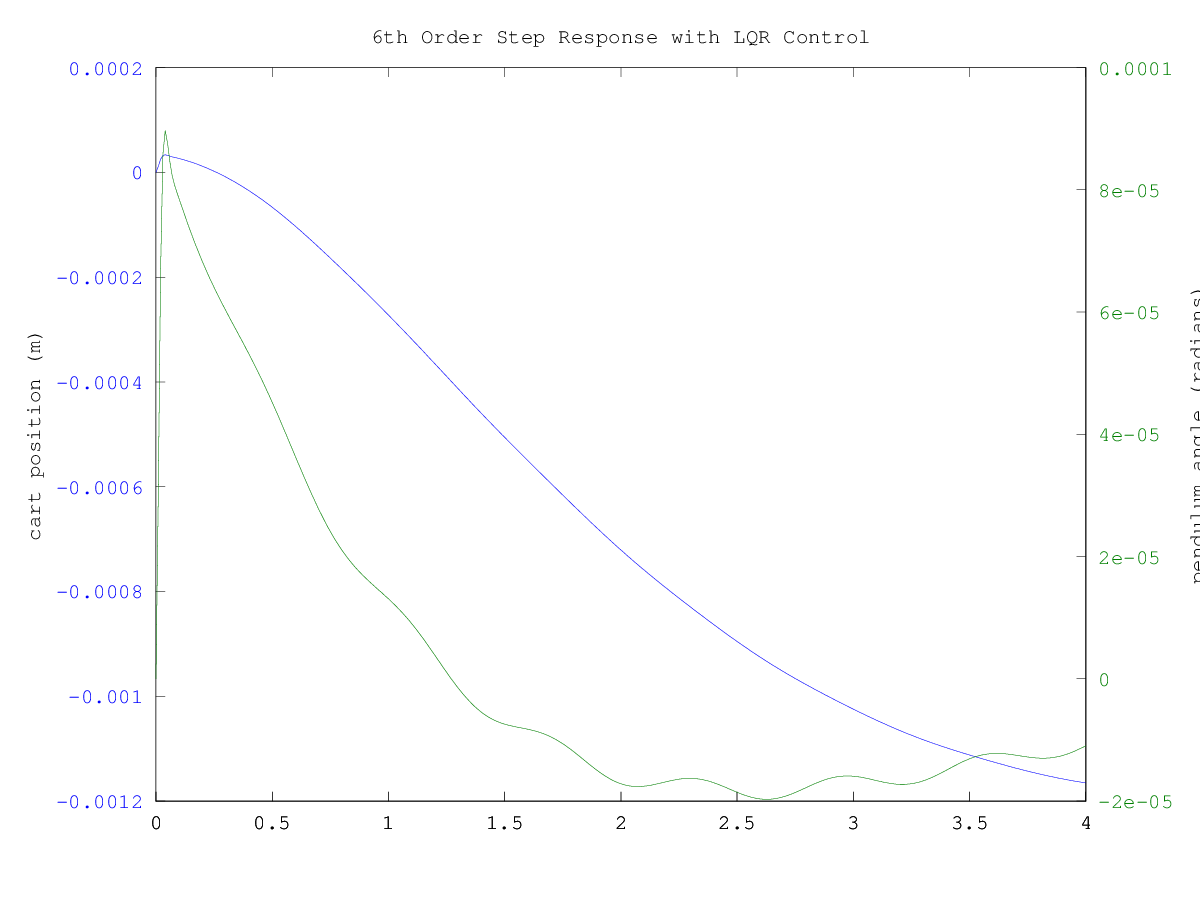
\includegraphics[width=0.5\linewidth]{6th_Order_Step_Response_with_LQR_Control}
	\label{fig:6osrwc}
}}
\caption{Step Response with LQR Control}
\end{figure}

\begin{figure}
\centering
\subfloat[4th Order]{{
	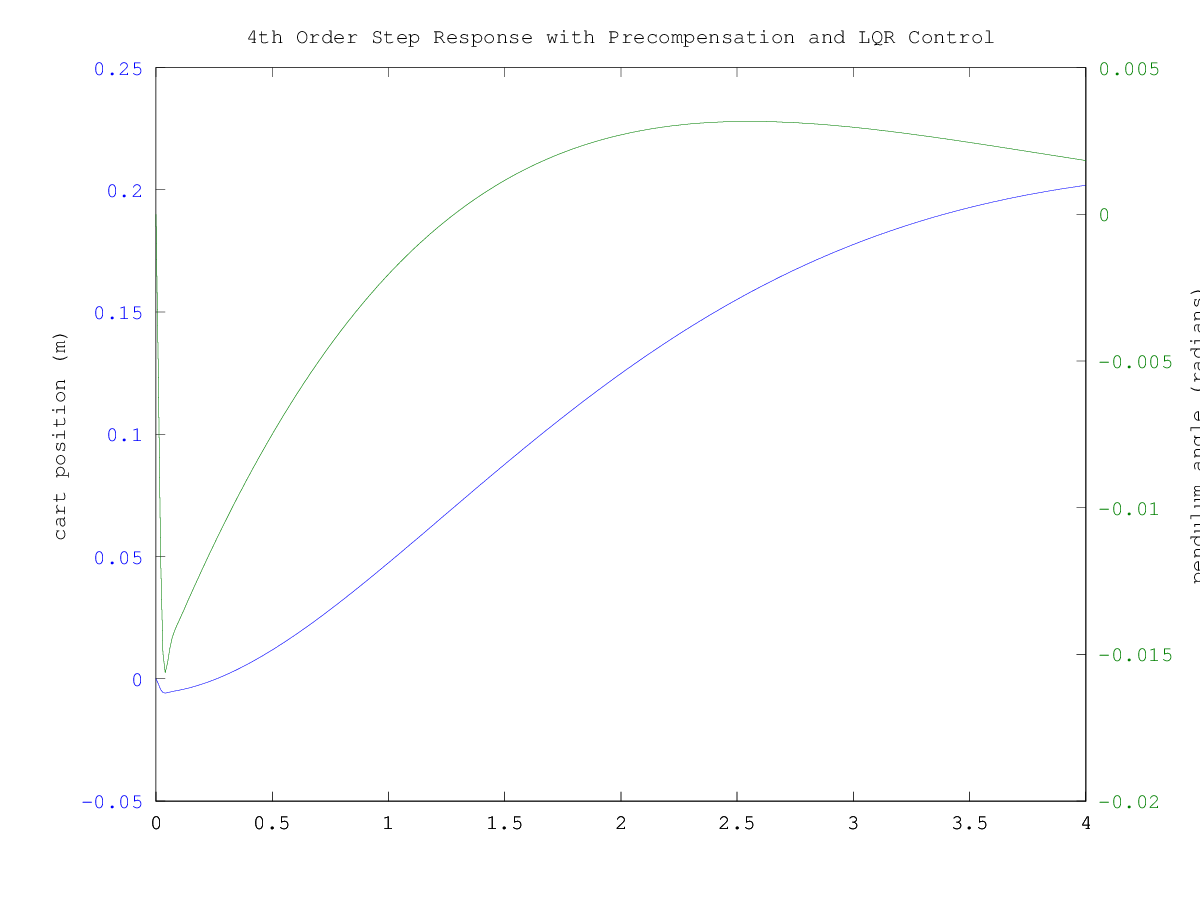
\includegraphics[width=0.5\linewidth]{4th_Order_Step_Response_with_Precompensation_and_LQR_Control}
	\label{fig:4osrwpc}
}}
\subfloat[6th Order]{{
	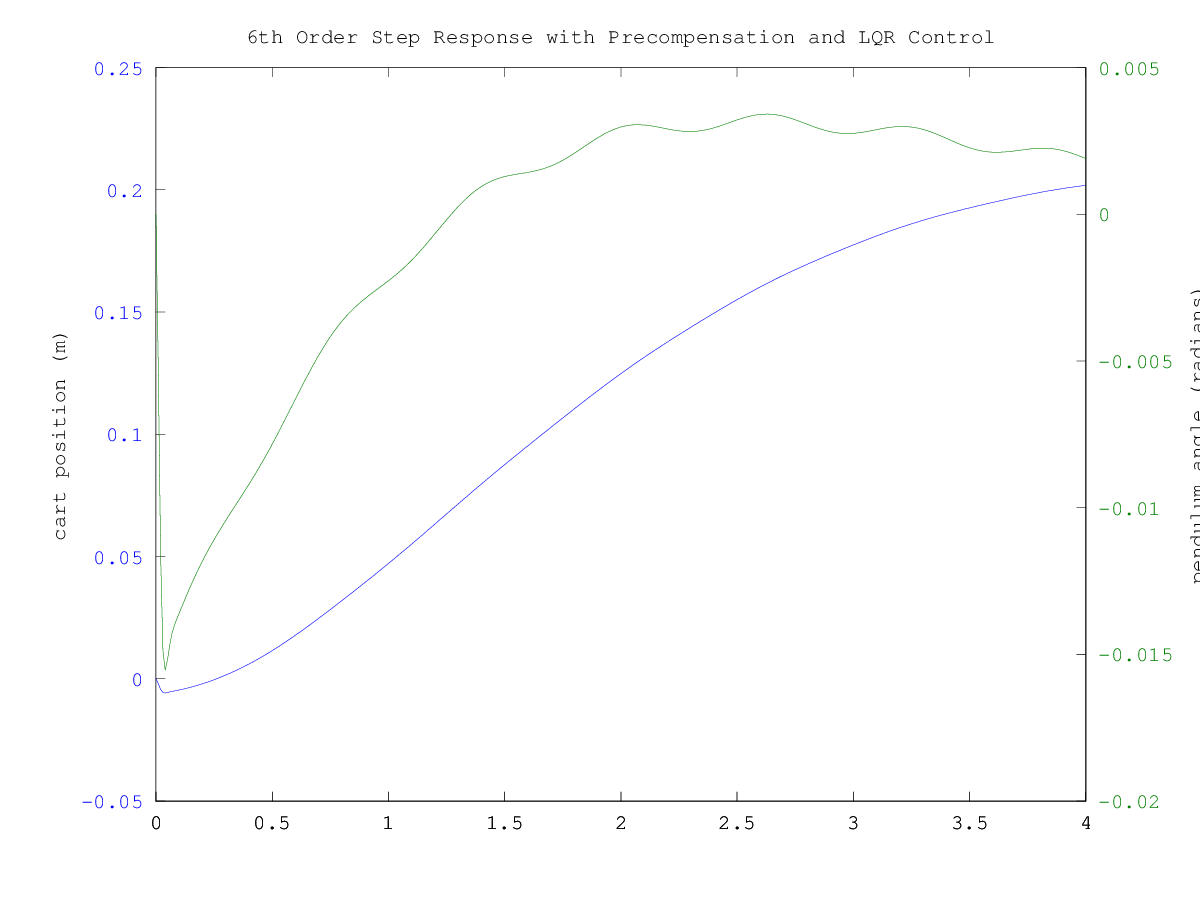
\includegraphics[width=0.5\linewidth]{6th_Order_Step_Response_with_Precompensation_and_LQR_Control}
	\label{fig:6osrwpc}
}}
\caption{Step Response with Precompensation and LQR Control}
\end{figure}

However, we don't have sensors for all of the states of these systems. We are only measuring the cart position and the pendulum angles. Figure \ref{fig:4osrwsfc} and \ref{fig:6osrwsfc} show the result when using a full-order observer. It is very close to what happened when using the actual state measurements in simulation.

\begin{figure}
\centering
\subfloat[4th Order]{{
	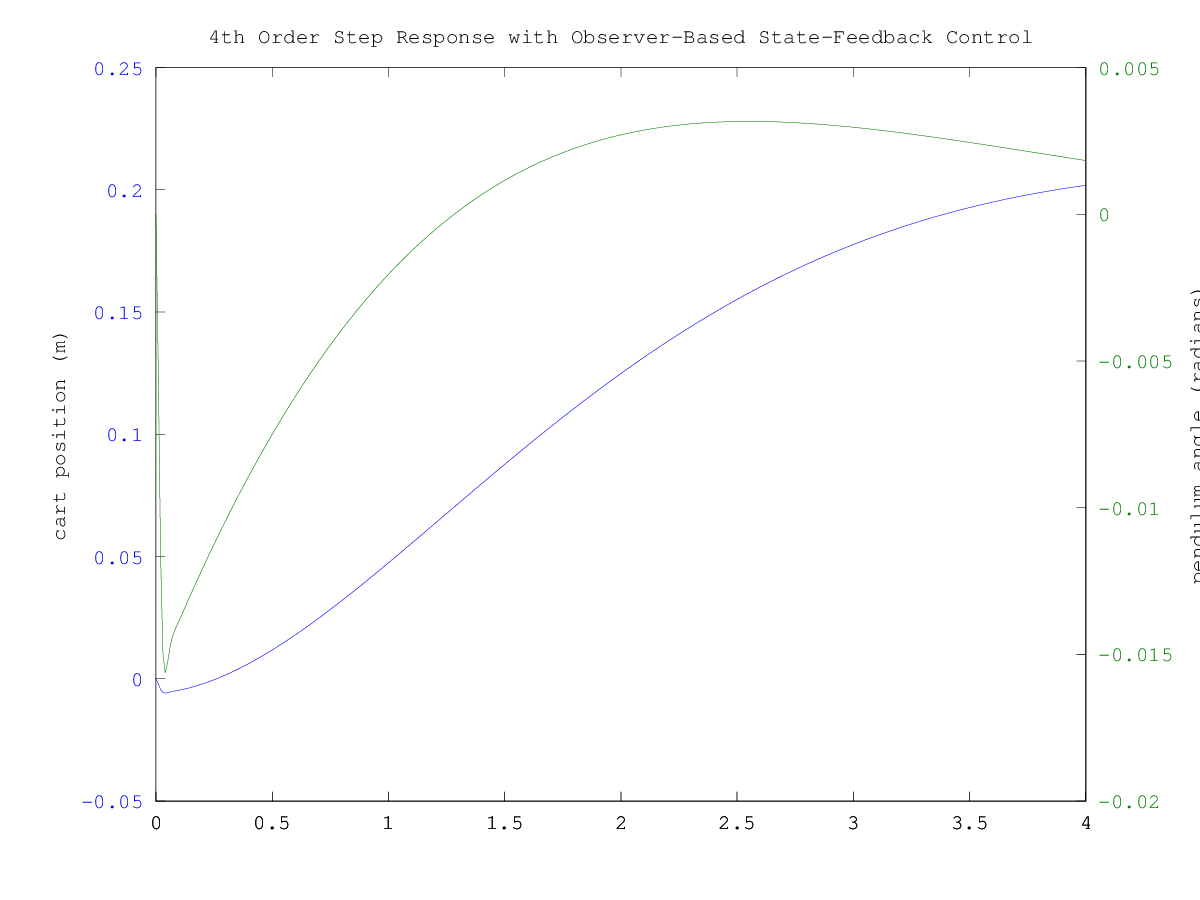
\includegraphics[width=0.5\linewidth]{4th_Order_Step_Response_with_Observer-Based_State-Feedback_Control}
	\label{fig:4osrwsfc}
}}
\subfloat[6th Order]{{
	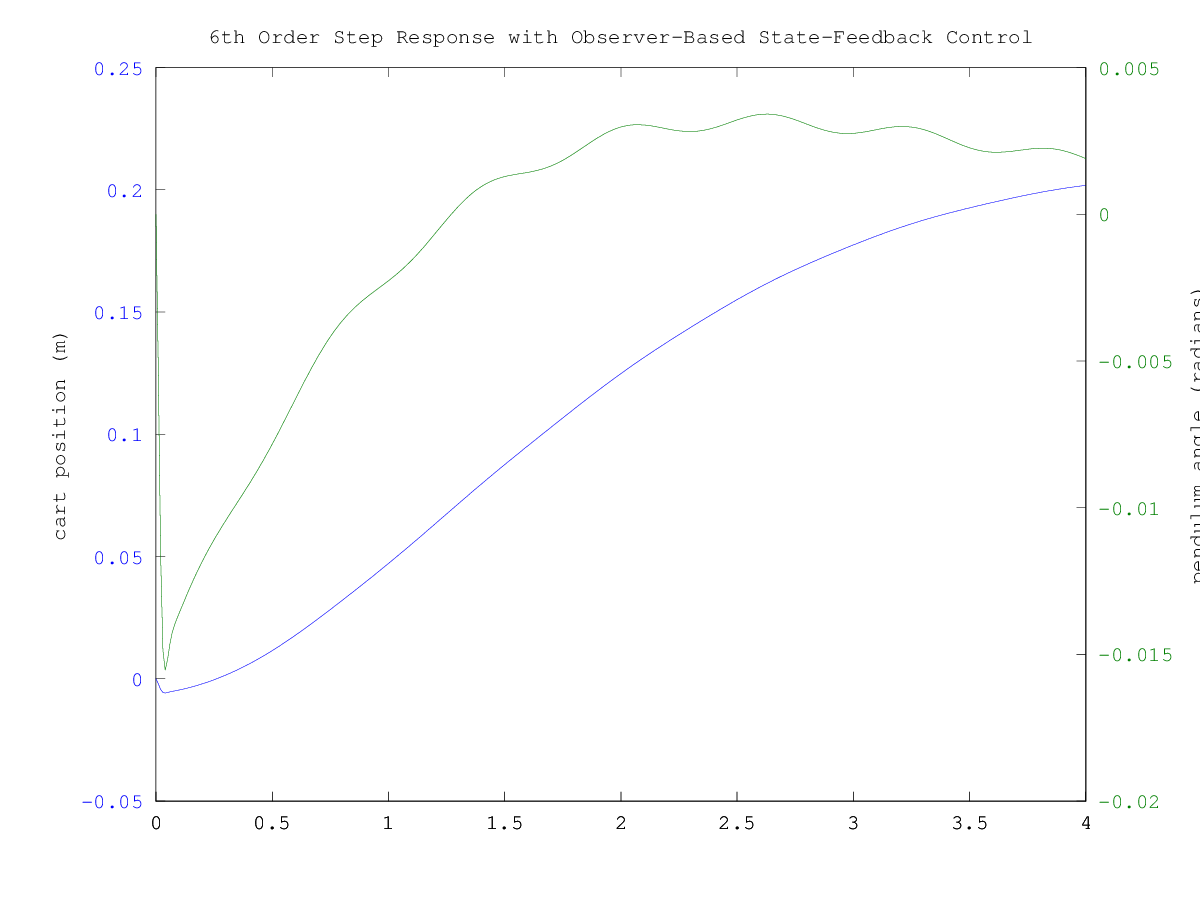
\includegraphics[width=0.5\linewidth]{6th_Order_Step_Response_with_Observer-Based_State-Feedback_Control}
	\label{fig:6osrwsfc}
}}
\caption{Step Response with Observer Based State Feedback Control}
\end{figure}

When we do this on the inverted pendulum in the real world, we will be doing it digitally, so we need to discretize our system. We are doing this with \textit{c2d} in Octave. To verify that our sampling rate won't cause issues, we can run the simulation on this discrete system. If the sampling rate is too low, the effect will be visible on these plots.

\begin{figure}
\centering
\subfloat[4th Order]{{
	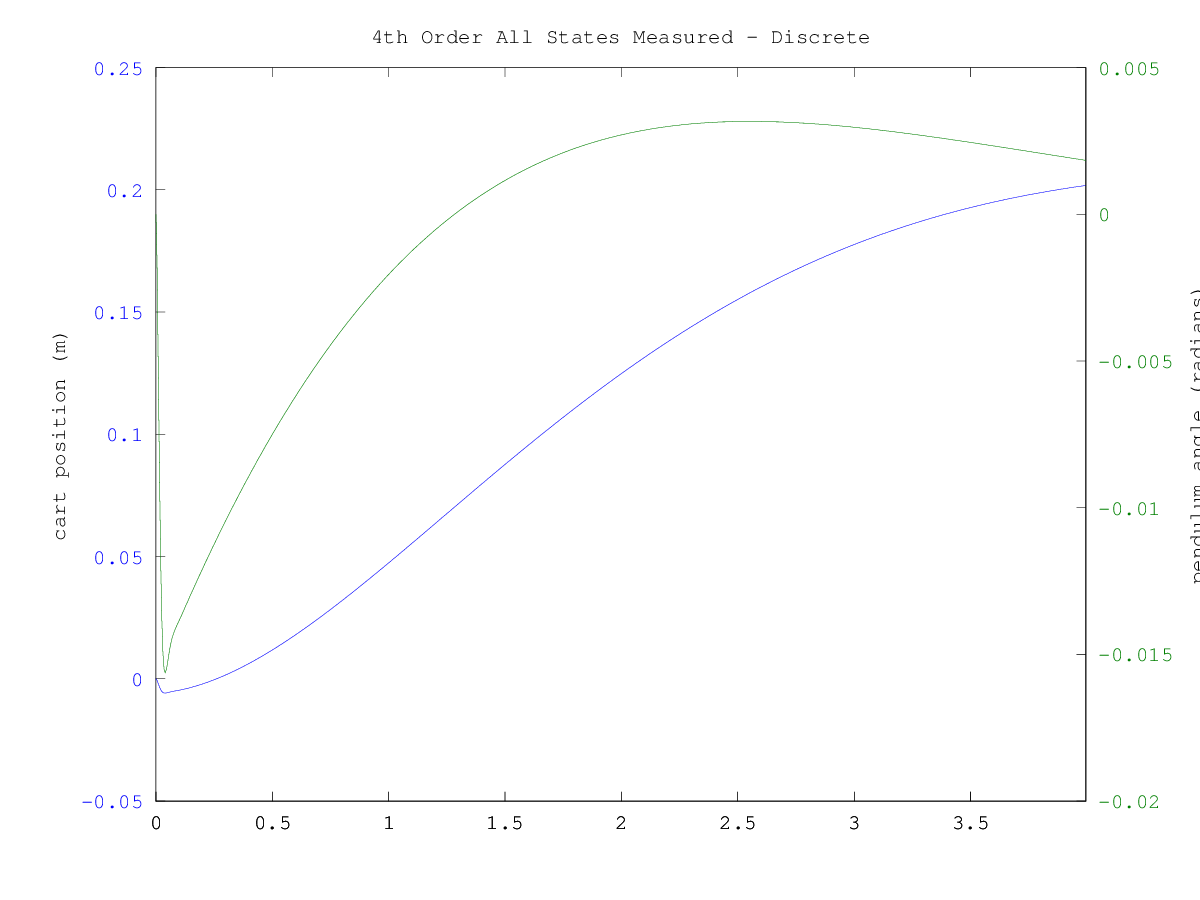
\includegraphics[width=0.5\linewidth]{4th_Order_All_States_Measured_Discrete}
	\label{fig:4oasmd}
}}
\subfloat[6th Order]{{
	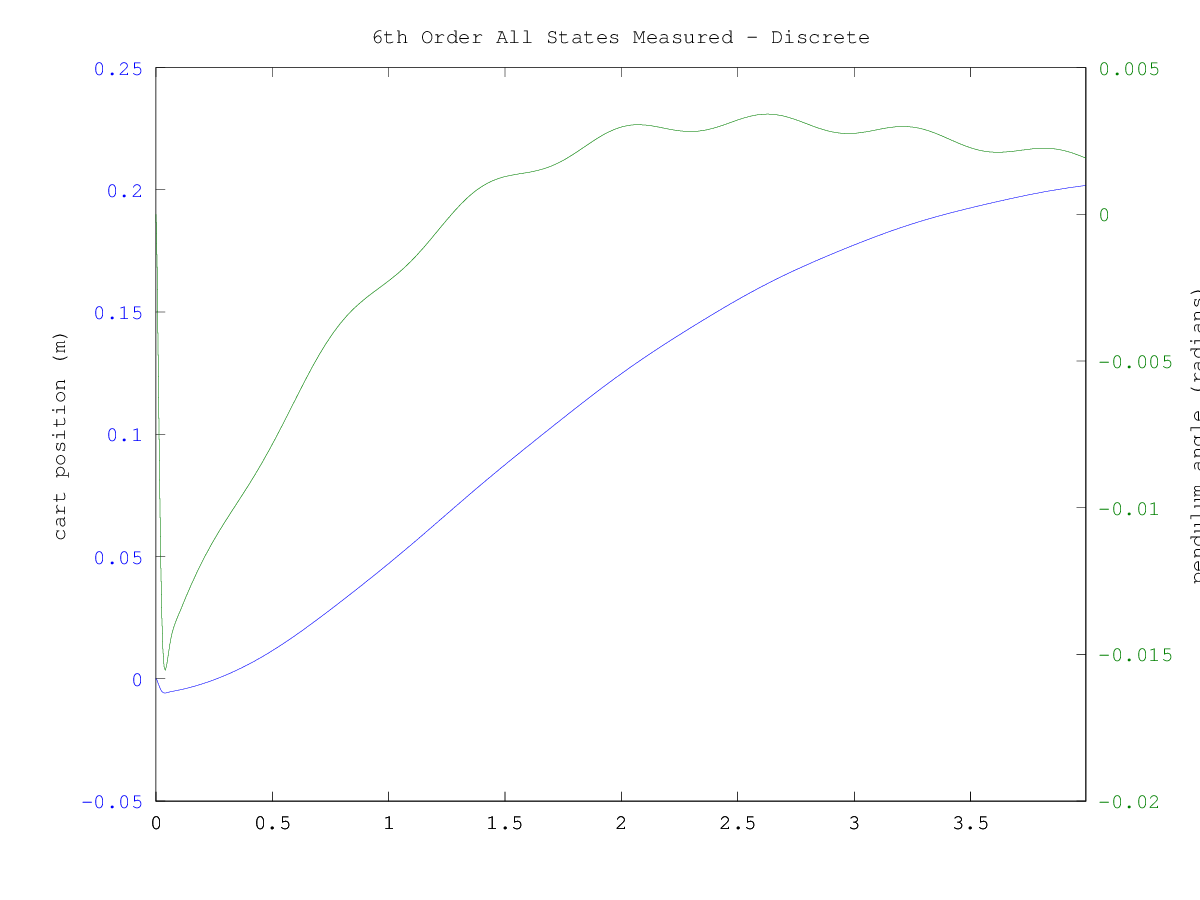
\includegraphics[width=0.5\linewidth]{6th_Order_All_States_Measured_Discrete}
	\label{fig:6oasmd}
}}
\caption{Discrete: All States Measured}
\end{figure}

Next, Figure \ref{fig:4osmed} and \ref{fig:6osed} show using our discretized estimator and also adding some Gaussian noise to our measurements to make this more realistic since the actual sensors might not have perfect readings.

\begin{figure}
\centering
\subfloat[4th Order]{{
	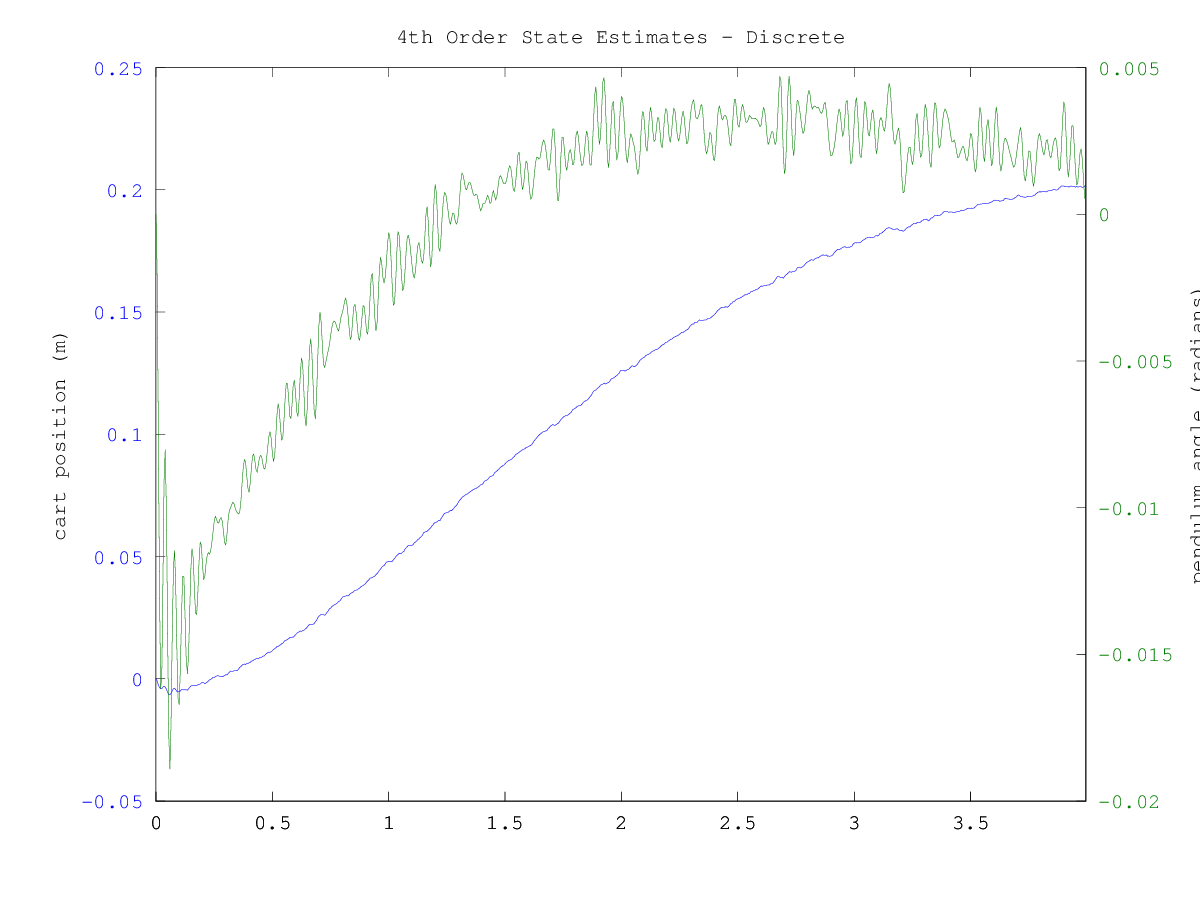
\includegraphics[width=0.5\linewidth]{4th_Order_State_Esimates_Discrete}
	\label{fig:4osmed}
}}
\subfloat[6th Order]{{
	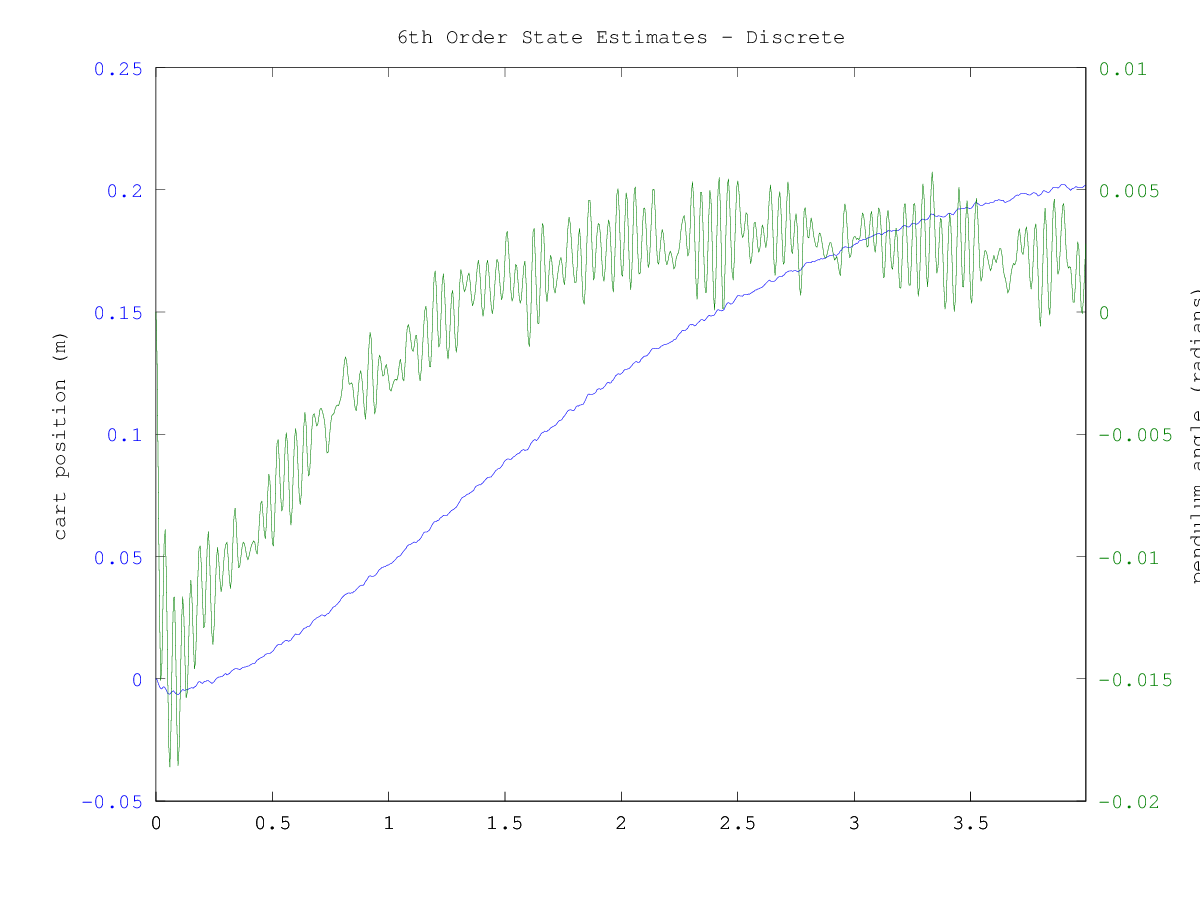
\includegraphics[width=0.5\linewidth]{6th_Order_State_Esimates_Discrete}
	\label{fig:6osed}
}}
\caption{Discrete: All State Estimations}
\end{figure}

Since we are dealing with a real motor and power supply, there are limits to what voltage we can apply to the motor. Figure \ref{fig:4ovo} and \ref{fig:6ovo} show what voltage is output to the motor from our system in simulation. This will allow us to see if we are driving the motor too hard, which will be visible on this plot as a square wave oscillating between the max and min output voltages.

\begin{figure}
\centering
\subfloat[4th Order]{{
	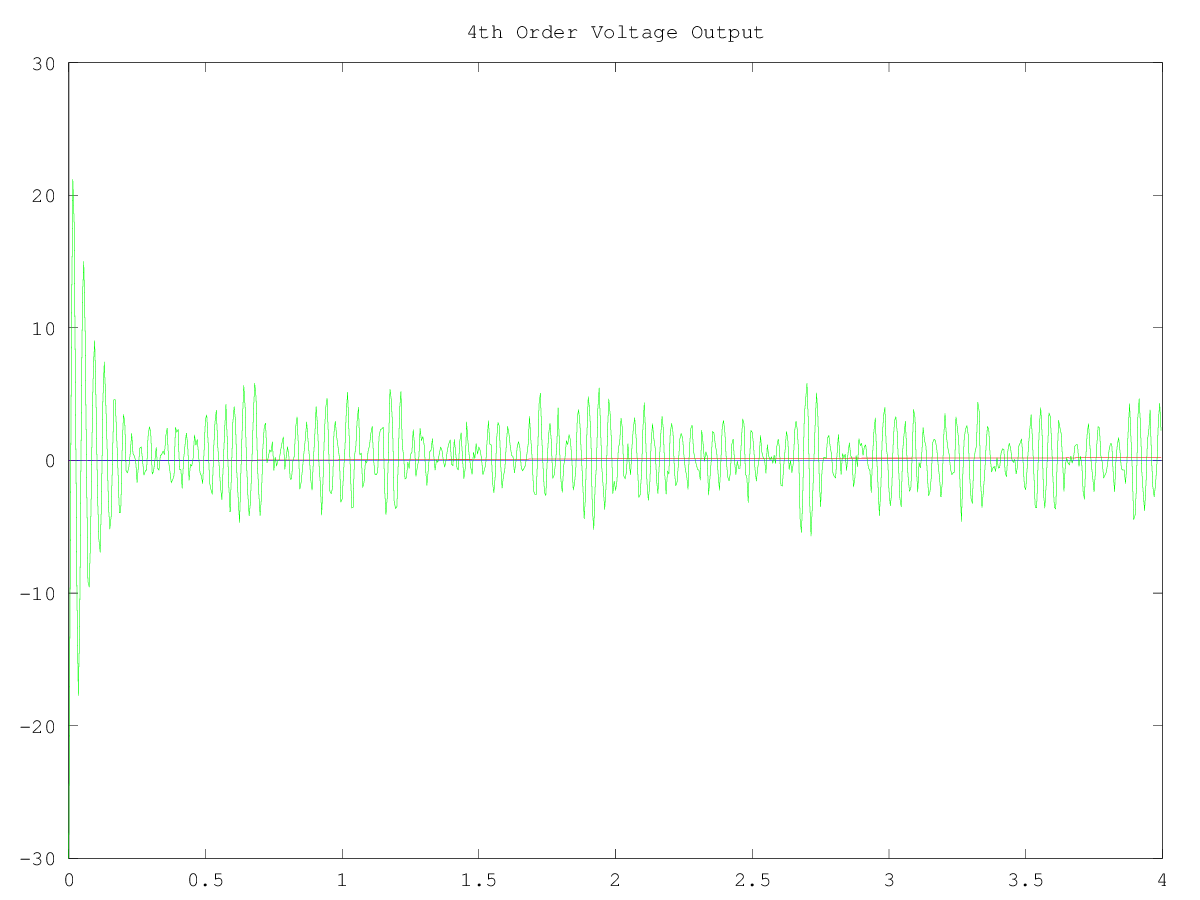
\includegraphics[width=0.5\linewidth]{4th_Order_Voltage_Output}
	\label{fig:4ovo}
}}
\subfloat[6th Order]{{
	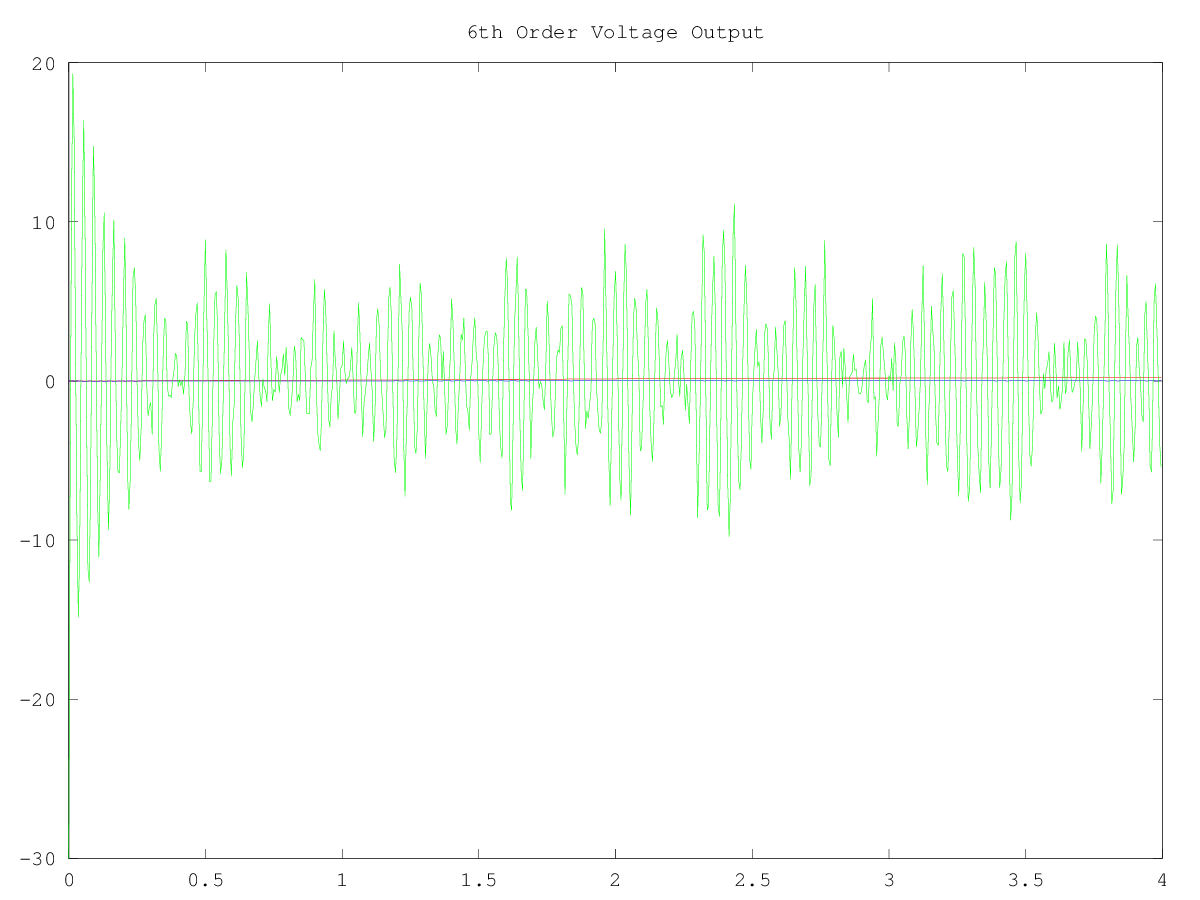
\includegraphics[width=0.5\linewidth]{6th_Order_Voltage_Output}
	\label{fig:6ovo}
}}
\caption{Discrete: Voltage Output to Motor}
\end{figure}

We wanted to estimate our states since our full-order observer in our test runs didn't quite match reality. Thus we tried a Kalman-like unbiased FIR filter as shown in Figure \ref{fig:4ufir} and \ref{fig:6ufir}. However, more work is required on this to get correct state estimates.

\begin{figure}
\centering
\subfloat[4th Order]{{
	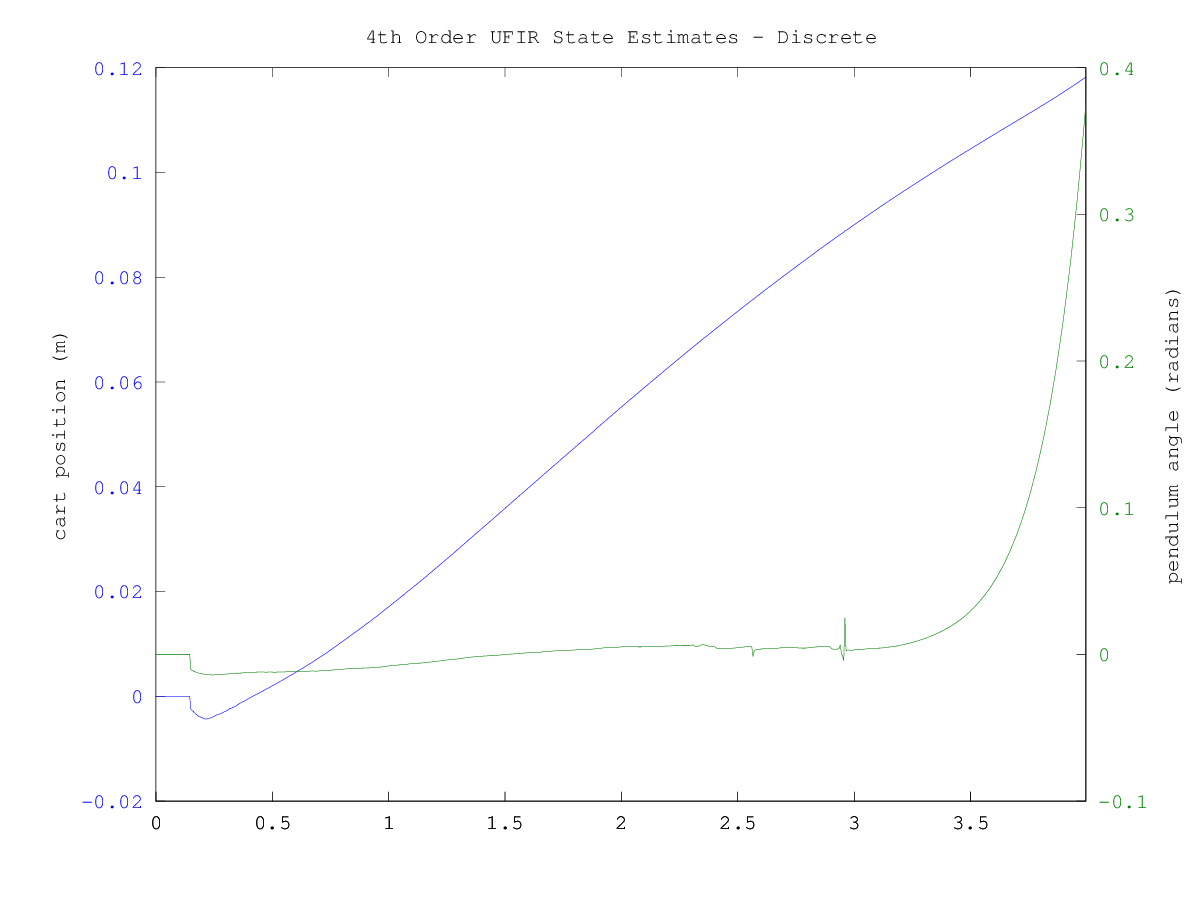
\includegraphics[width=0.5\linewidth]{4th_Order_UFIR_State_Estimates_Discrete}
	\label{fig:4ufir}
}}
\subfloat[6th Order]{{
	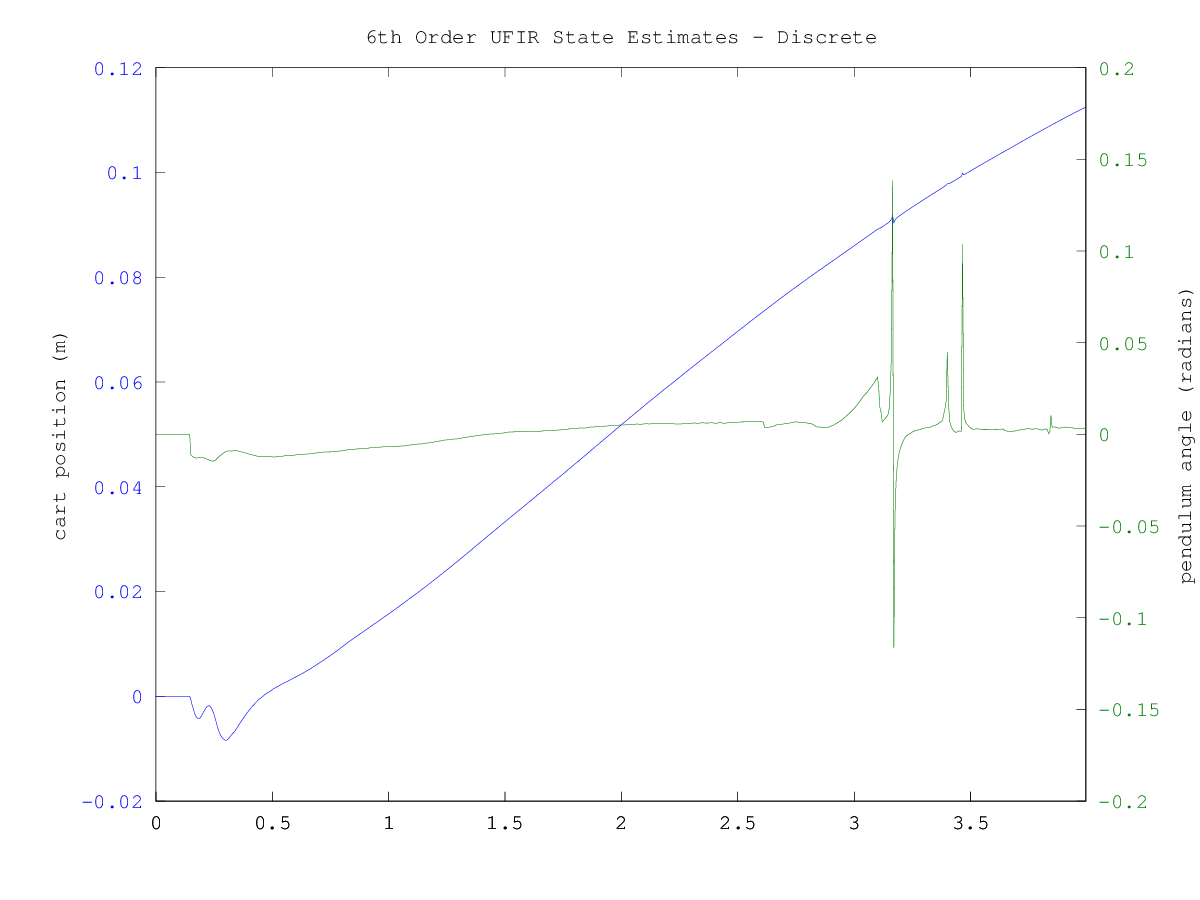
\includegraphics[width=0.5\linewidth]{6th_Order_UFIR_State_Estimates_Discrete}
	\label{fig:6ufir}
}}
\caption{Discrete: UFIR State Estimates}
\end{figure}

Figure \ref{fig:c4oe} and \ref{fig:c4om} use the voltage level we were given in the list of system parameters, which was 20 V. These graphs have the correct radius for the motor. They show the long pendulum staying inverted for approximately 12 seconds.

\begin{figure}
\centering
\subfloat[Estimated]{{
	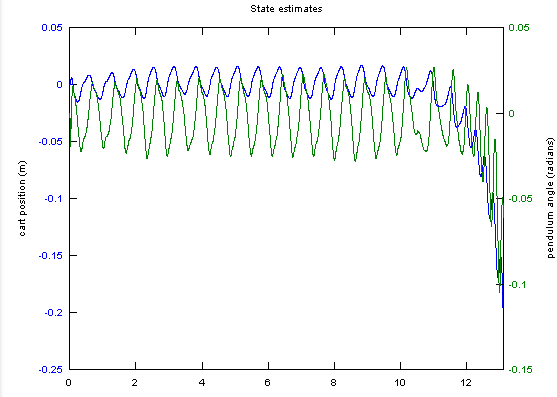
\includegraphics[width=0.5\linewidth]{Correct4thOrder_estimated}
	\label{fig:c4oe}
}}
\subfloat[Measured]{{
	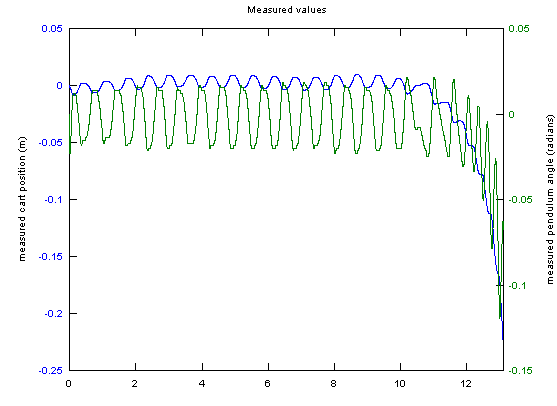
\includegraphics[width=0.5\linewidth]{Correct4thOrder_measured}
	\label{fig:c4om}
}}
\caption{4th Order With 20V Max Voltage}
\end{figure}

Figure \ref{fig:c6oe}, \ref{fig:c6om}, \ref{fig:c6ole}, and \ref{fig:c6olm} use the voltage level we measured on the output of the motor, which was 30 V. The state estimations are far from the actual values we measured as shown in Figure \ref{fig:c6om} and \ref{fig:c6olm}. The 6th order system keeps the pendulum centered around a position of $x=0$ much more consistently than the 4th order system in our tests. This is what we would think should happen since the 6th order system takes into account the small pendulum hanging down. However, note that we used the small angle approximation for the both pendulums, so if the small pendulum is swinging wildly, then our state estimates might not follow as close to reality as we would hope.

\begin{figure}
\centering
\subfloat[Estimated]{{
	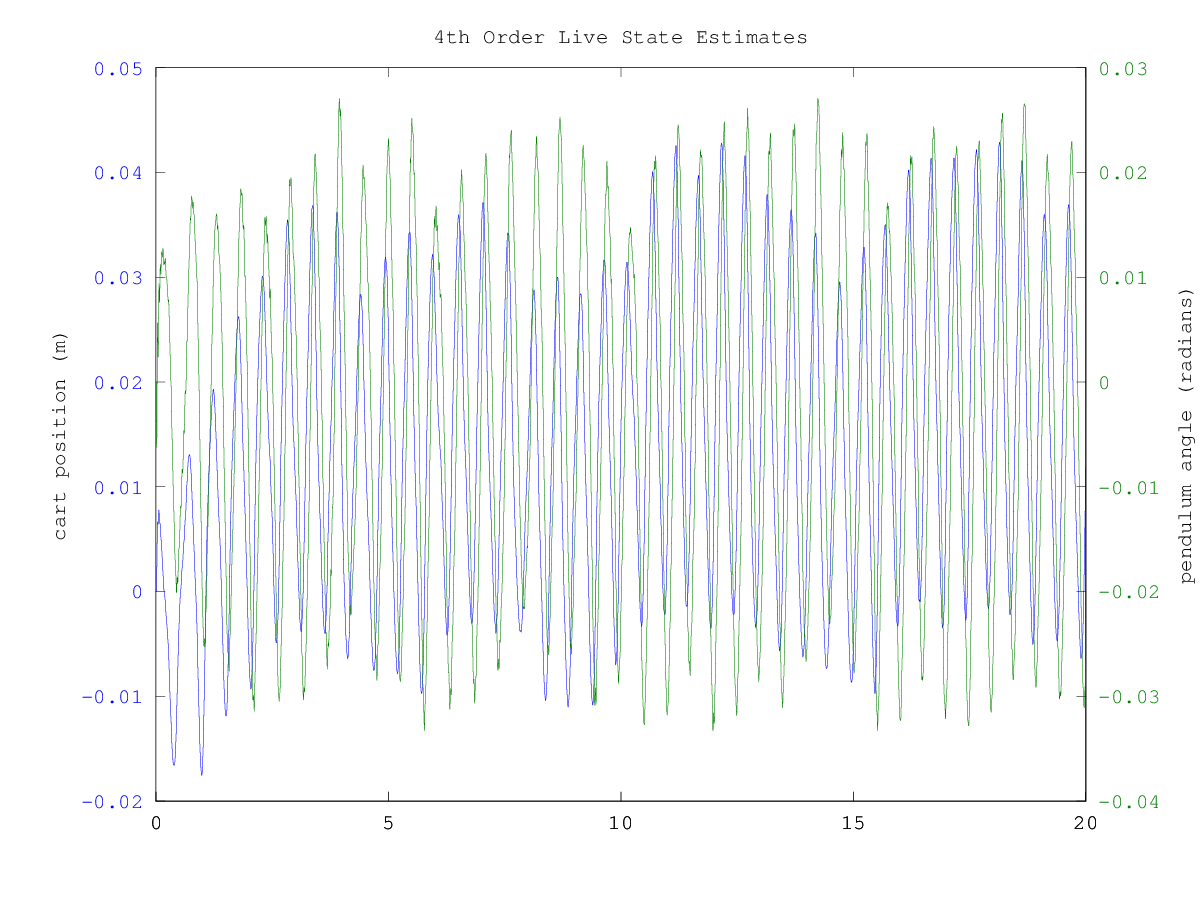
\includegraphics[width=0.5\linewidth]{4th_Order_Live_State_Estimates}
	\label{fig:c6oe}
}}
\subfloat[Measured]{{
	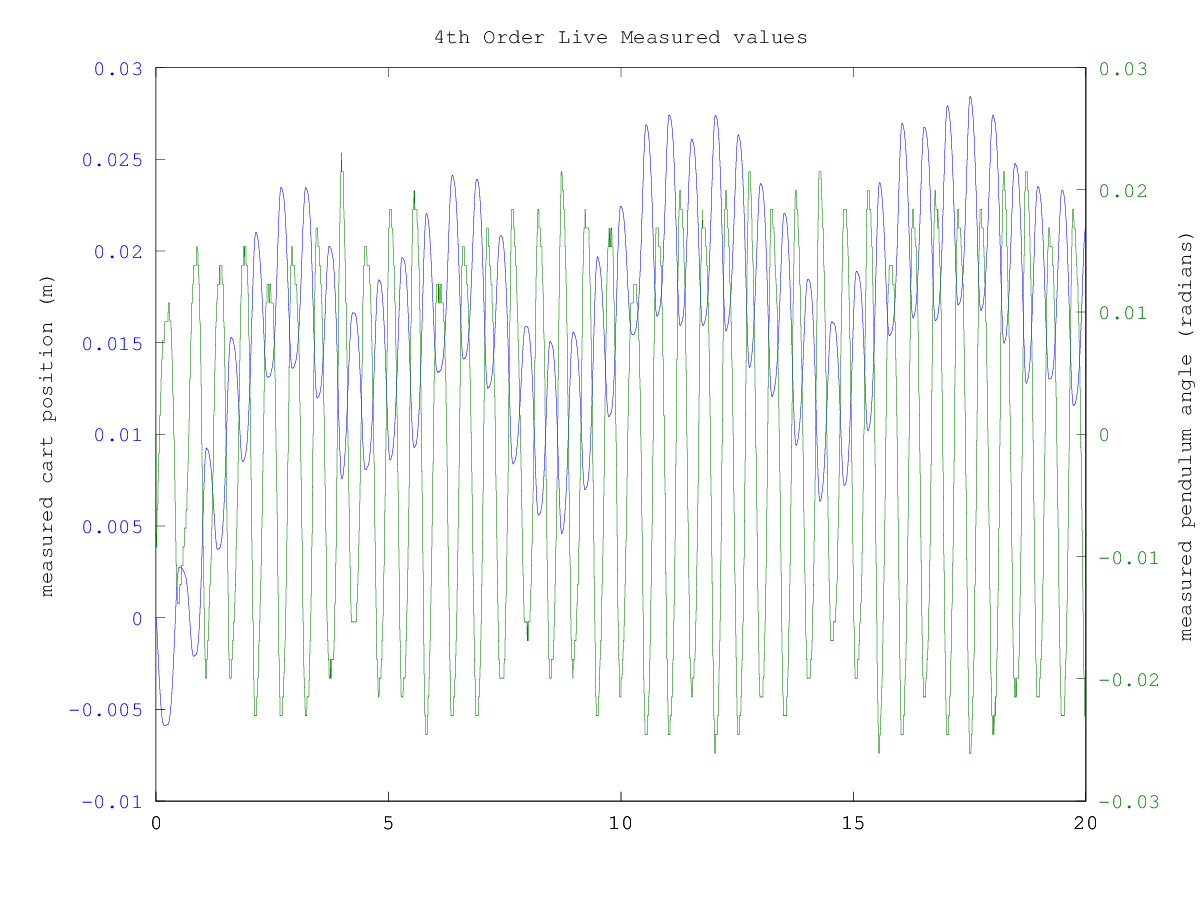
\includegraphics[width=0.5\linewidth]{4th_Order_Live_Measured_Values}
	\label{fig:c6om}
}}
\caption{4th Order With 30V Max Voltage}
\end{figure}

\begin{figure}
\centering
\subfloat[Estimated]{{
	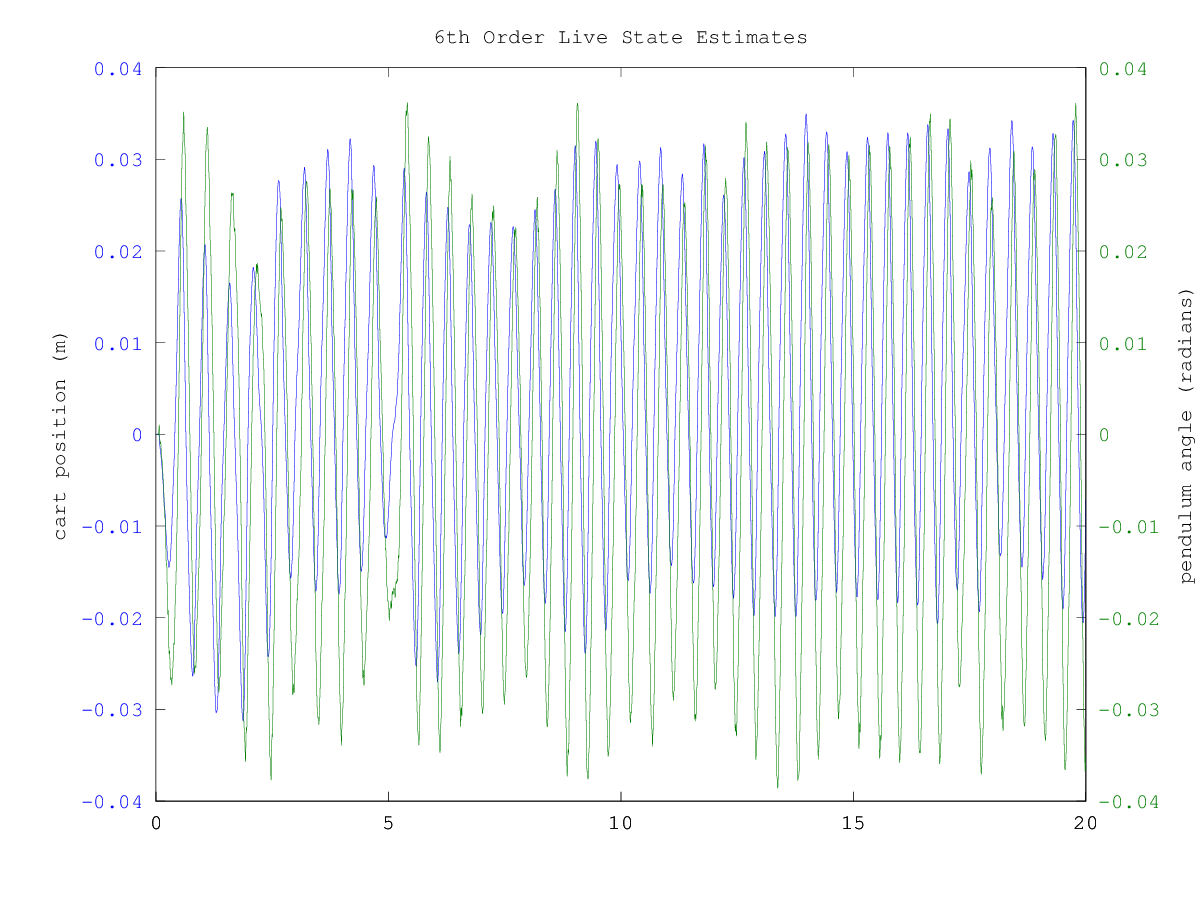
\includegraphics[width=0.5\linewidth]{6th_Order_Live_State_Estimates}
	\label{fig:c6ole}
}}
\subfloat[Measured]{{
	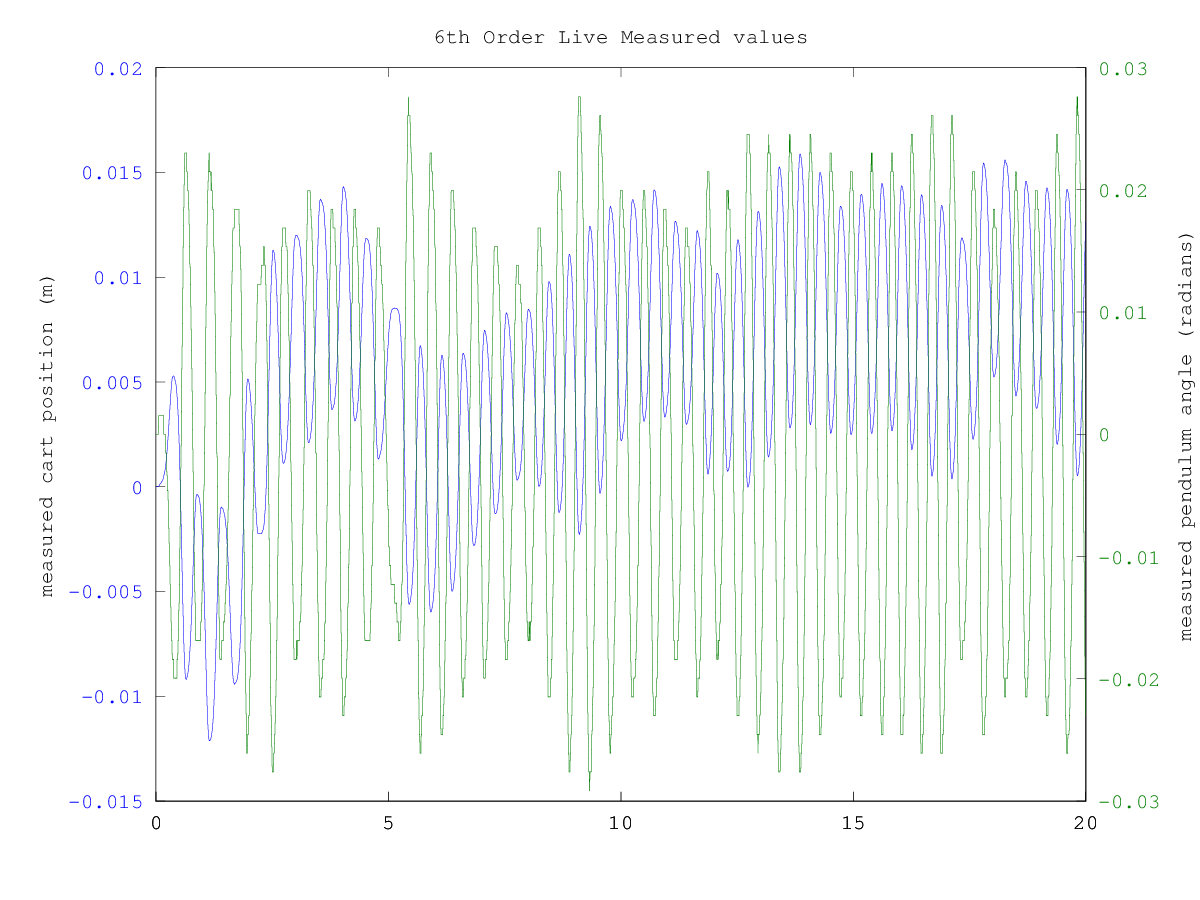
\includegraphics[width=0.5\linewidth]{6th_Order_Live_Measured_Values}
	\label{fig:c6olm}
}}
\caption{6th Order With 30V Max Voltage}
\end{figure}

In addition, we found that the program that is generally used to demo the inverted pendulum, which was created by Andrew Roth, multiplied the measured motor angle by $r_d$ in two places, which is the same as setting $r_d$ to be the square of what we would expect. When we made this alteration, both the 4th and 6th order system worked better. The correct value is $r_d = 0.0127$ m, but in this case we used $r_d = 0.00016129$ m. However, the system acted similarly when we used the correct radius and used $Maxvoltage = 30$ V instead of $Maxvoltage = 20$ V.

\section{Future Work}
\begin{itemize}
\item Experiment with the $Q$ matrix for LQR trying weighting all of the states instead of just $x$ and $\theta$.
\item Fix the UFIR state estimates. This requires figuring out why the algorithm depends on $inv(A*F*A')$, which is a problem since all of our $A$ matrices are non-invertible. An alternative is using the Octave package called ALS, which uses a Kalman filter and provides a method to determine the variances. However, in theory, the UFIR will outperform the Kalman filter in the majority of cases; though, it is more computationally intensive.
\item We could verify that the system parameters we are using are correct. For example, we could measure the velocity of the motor when we spin the motor at a certain velocity by an external force, which would allow us to check the motor's $K$ value.
\item Instead of verifying system parameters, we could also do system identification to determine all the system parameters by providing white noise as the input and doing a best fit.
\item While it won't necessarily provide any improvement, it would be fairly simple to take the \href{https://github.com/floft/PIDinStateSpace}{PID in State-Space form} equations to test a PID controller with our existing code.
\item We could try getting the short pendulum to stay up while the long one hangs down, or we could work more on getting both pendulums to stay up simultaneously.
\end{itemize}

\section{References}
\begin{itemize}
\item \href{https://www.researchgate.net/publication/233854533_A_Kalman-like_FIR_estimator_ignoring_noise_and_initial_conditions}{A Kalman-like FIR estimator ignoring noise and initial conditions}
\item \href{http://engagedscholarship.csuohio.edu/cgi/viewcontent.cgi?article=1214&context=enece_facpub}{Iterative Unbiased FIR State Estimation: A Review of Algorithms}
\item \href{http://jbrwww.che.wisc.edu/software/als/index.html}{ALS Octave Package}
\item \href{http://jbrwww.che.wisc.edu/tech-reports/twmcc-2007-02.pdf}{Explanation of Autocovariance Least-Squares (ALS) Method}
\end{itemize}

\end{document}
